\section{Gegen\"uberstellung der Simulations und Messergebnisse}\label{sec:gegenueberst}
Ausgehend von den beschriebenen Modellierungsschritten kann nun eine sichere Evaluierung der Kurzschlussanordnungen angesetzt werden. Dabei k\"onnen die Messungen sowie das Simulationsmodell zur Kreuzvalidierung verwendet werden, sodass Mess- und Simulationsfehler weitestgehend auszuschlie\ss{}en sind. Dazu wurde das Simulationsmodell, nach den in Absatz~\ref{chap:simulation} versehenen Anpassungen zun\"achst einmal zur Referenz mit den Messungen verglichen. Dazu wird die Testbox ohne Ringkern, jedoch mit fertigem Halterungsaufbau gegen\"ubergestellt. Abbildung~\ref{fig:boxpolycross} zeigt diese Gegen\"uberstellung.

\begin{figure}[htb]
	\centering
	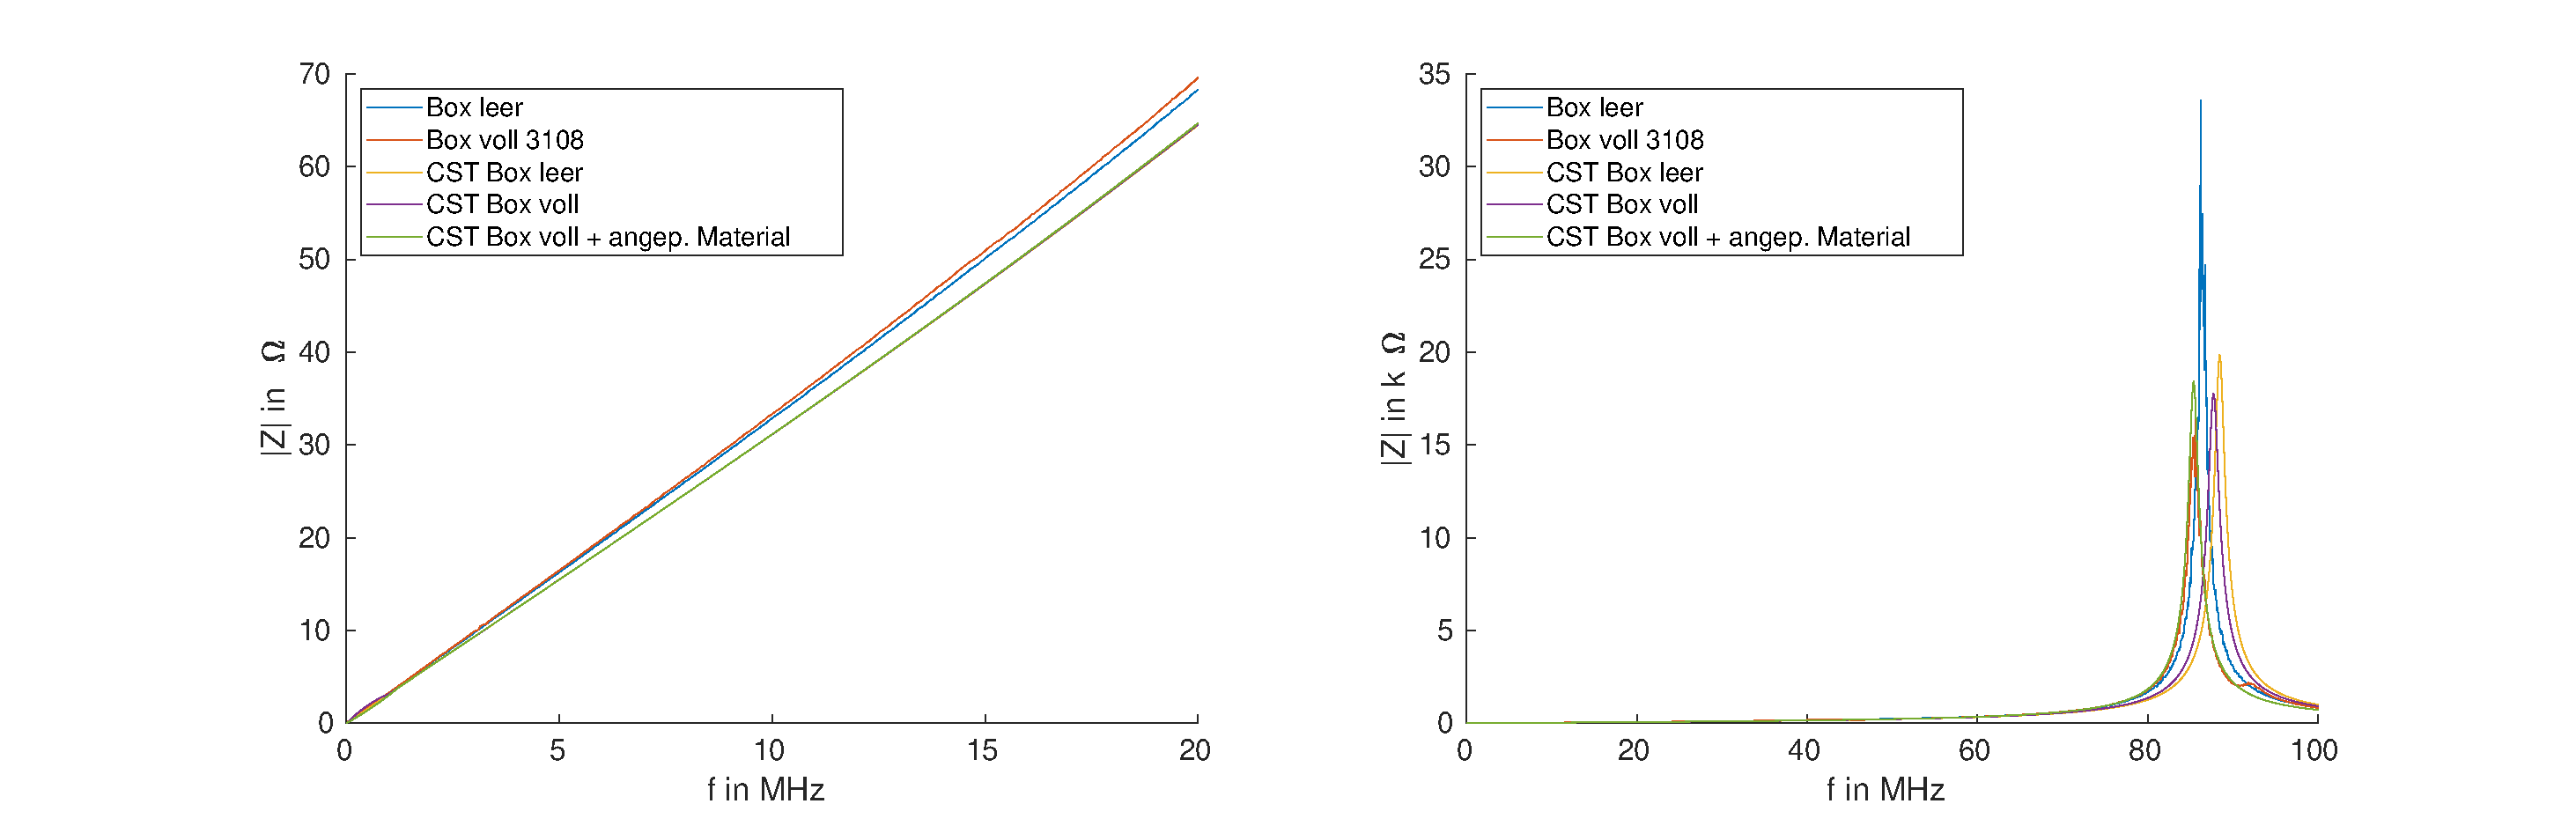
\includegraphics[width=\textwidth]{measurement_simulation_emptybox}
	\caption{Gegen\"uberstellung der Simulation der Box mit Halterung aus Kreuz und Polygon zur entsprechenden Messung.}
	\label{fig:boxpolycross}
\end{figure}

Mit Hilfe von Abbildung~\ref{fig:boxpolycross} können zunächst Messung und Simulation auf Plausibilität überprüft werden.\\
Die Resonanzfrequenz $f_r = \frac{1}{2\pi \cdot \sqrt{LC}}$ eines LC-Schwingkreise sinkt mit steigendem $\varepsilon_r$, da hierdurch die Kapazität erhöht wird. Je mehr Einbauten der Testbox hinzugefügt werden, desto größer kann $\varepsilon_r$ einer Ersatzkapazit\"at angesehen werden, wodurch die Resonanz zu niedrigeren Frequenzen hin verschoben wird.\\
Außerdem zeigt die Abbildung, wie die Simulation durch die Veränderung von $\varepsilon_r$ der Holzkonstruktion mit der Messung besser in Übereinstimmung gebracht werden konnte. Es wurde hierbei vornehmlich $\varepsilon_r'$ variiert. Dieser Vorgehensweise liegt die Annahme zugrunde, dass das verwendete Material in der Testbox mit den für die Simulation hinterlegten Werten übereinstimmt.
\par
Als n\"achstes ist das Modell mit eingesetztem Ringkern zu evaluieren. Dazu wird der Ringkern f\"ur die Simulation auf der Position um den Trovidur Ring gelegt, um die reale Box genau abzubilden. Der Aufbau ist in Abbildung~\ref{fig:RKFeRingCST} gezeigt. Auch hierbei wird wieder die gemessene Impedanz an der Einkopplung direkt mit der Impedanz aus der Simulation gegen\"ubergestellt. Diese Auswertung ist in Abbildung~\ref{fig:boxpolycrossrk} zu sehen.



\newpage



\begin{figure}[htb]
	\centering
	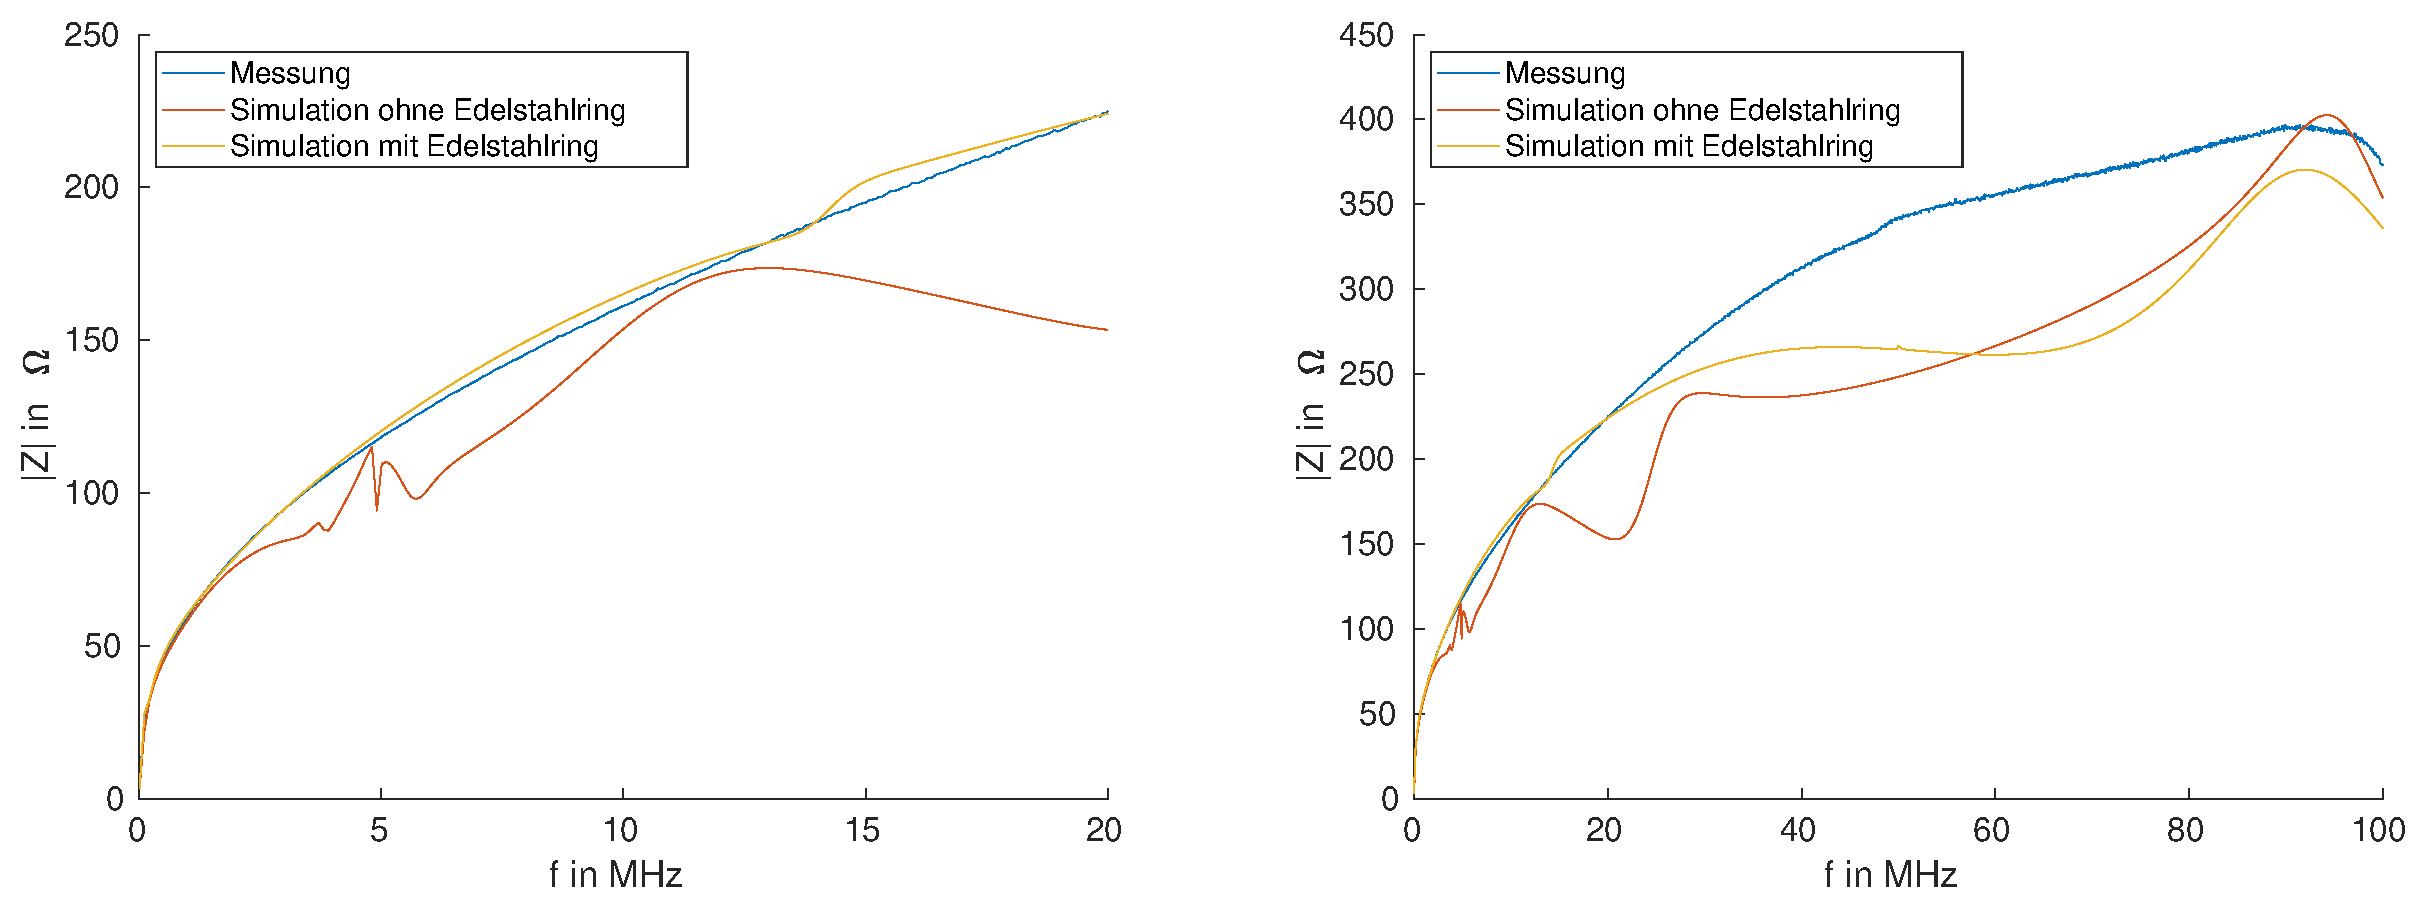
\includegraphics[width=\textwidth]{Zges_RK_SimMeas}
	\caption{Gegen\"uberstellung der gemessenen, mit der simulierten Ringkernimpedanz ohne Kurzschl\"usse}
	\label{fig:boxpolycrossrk}
\end{figure}

F\"ur die erste Simulation wurde sowohl der Ringkern als auch die Halterung dissipativ modelliert. In den CST-Einstellungen wurde das Adaptive Mesh Refinement ausgeschaltet und eine fixe Meshgr\"o\ss{}e von rund $3\cdot10^6$ Meshzellen verwendet. Die Simulation zeigt eine gewisse Welligkeit und nach wie vor eine Abweichung zur Messung. Diese Abweichung konnte bis $\SI{20}{\mega\hertz}$ minimiert werden indem die Ringkernhaltung durch Edelstahl mit $\mu_r = 1$ modeliert.
Dieses Vorgehen wurde jedoch nicht für die weiteren Kurzschluss-Simulationen angewendet (siehe \ref{sec:rksimulation}). 
% \par
% Die Gegen\"uberstellung wird f\"ur alle in Abschnitt~\ref{sec:testbox} genannten Kurzschlussanordnungen in gleicher Form durchgef\"uhrt.
% Es zeigt sich schnell, dass insbesondere im niedrigen Frequenzbereich eine sehr geringe Abweichung zu erkennen ist. Die Mittlere Abweichung zwischen Simulation und Messung liegt unterhalb von $\SI{20}{\mega\hertz}$ bei nur 

% \todo[inline,color=red!30]{wert und ggf Rechnung einf\"ugen}.  
\par
Auch die Kurzschlussmessungen wurden mit der Simulation gegen\"ubergestellt. Zun\"achst wird die Anordnung mit nur einem Kurzschluss betrachtet. Insbesondere im Bereich bis $\SI{50}{\mega\hertz}$ ist eine hohe \"Ubereinstimmung zu sehen. Lediglich im h\"oheren Frequenzbereich, nahe der Resonanz, weichen Messung und Simulation voneinander ab. Abbildung~\ref{fig:boxpolycrossrk1ks} zeigt die Gegen\"uberstellung.

\begin{figure}[htb]
	\centering
	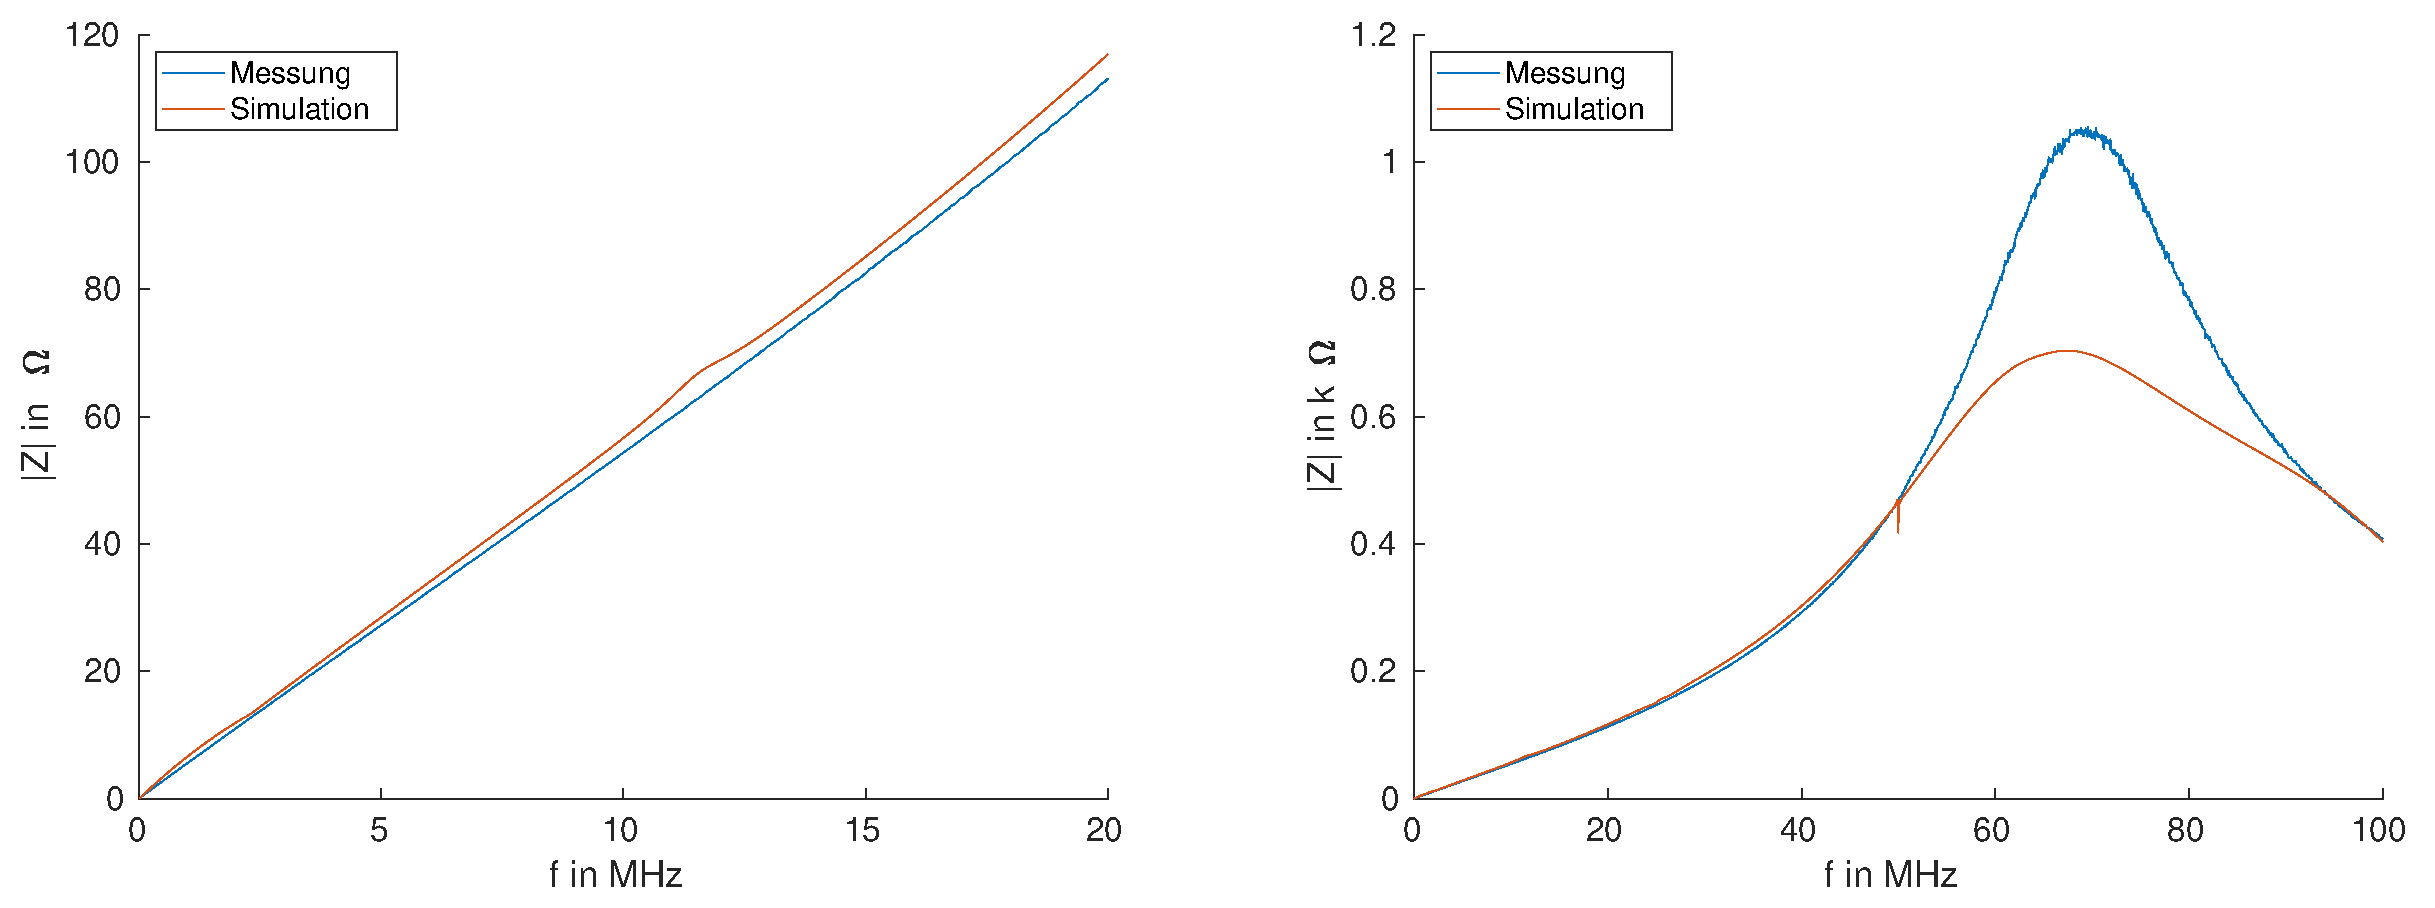
\includegraphics[width=\textwidth]{Z_ges_1KS_SimMeas}
	\caption{Gegen\"uberstellung der gemessenen, mit der simulierten Ringkernimpedanz f\"ur einen Kurzschluss.}
	\label{fig:boxpolycrossrk1ks}
\end{figure}



\newpage



Die Simulation der weiteren Kurzschl\"ussanordnungen zeigt, dass je mehr Kurzschlüsse simuliert werden, die Abweichung zur Messung steigt. Abbildung~\ref{fig:boxpolycrossrk7ks} zeigt diesen Effekt beispielhaft f\"ur eine Anzahl von sieben Kurzschl\"ussen.

\begin{figure}[htb]
	\centering
	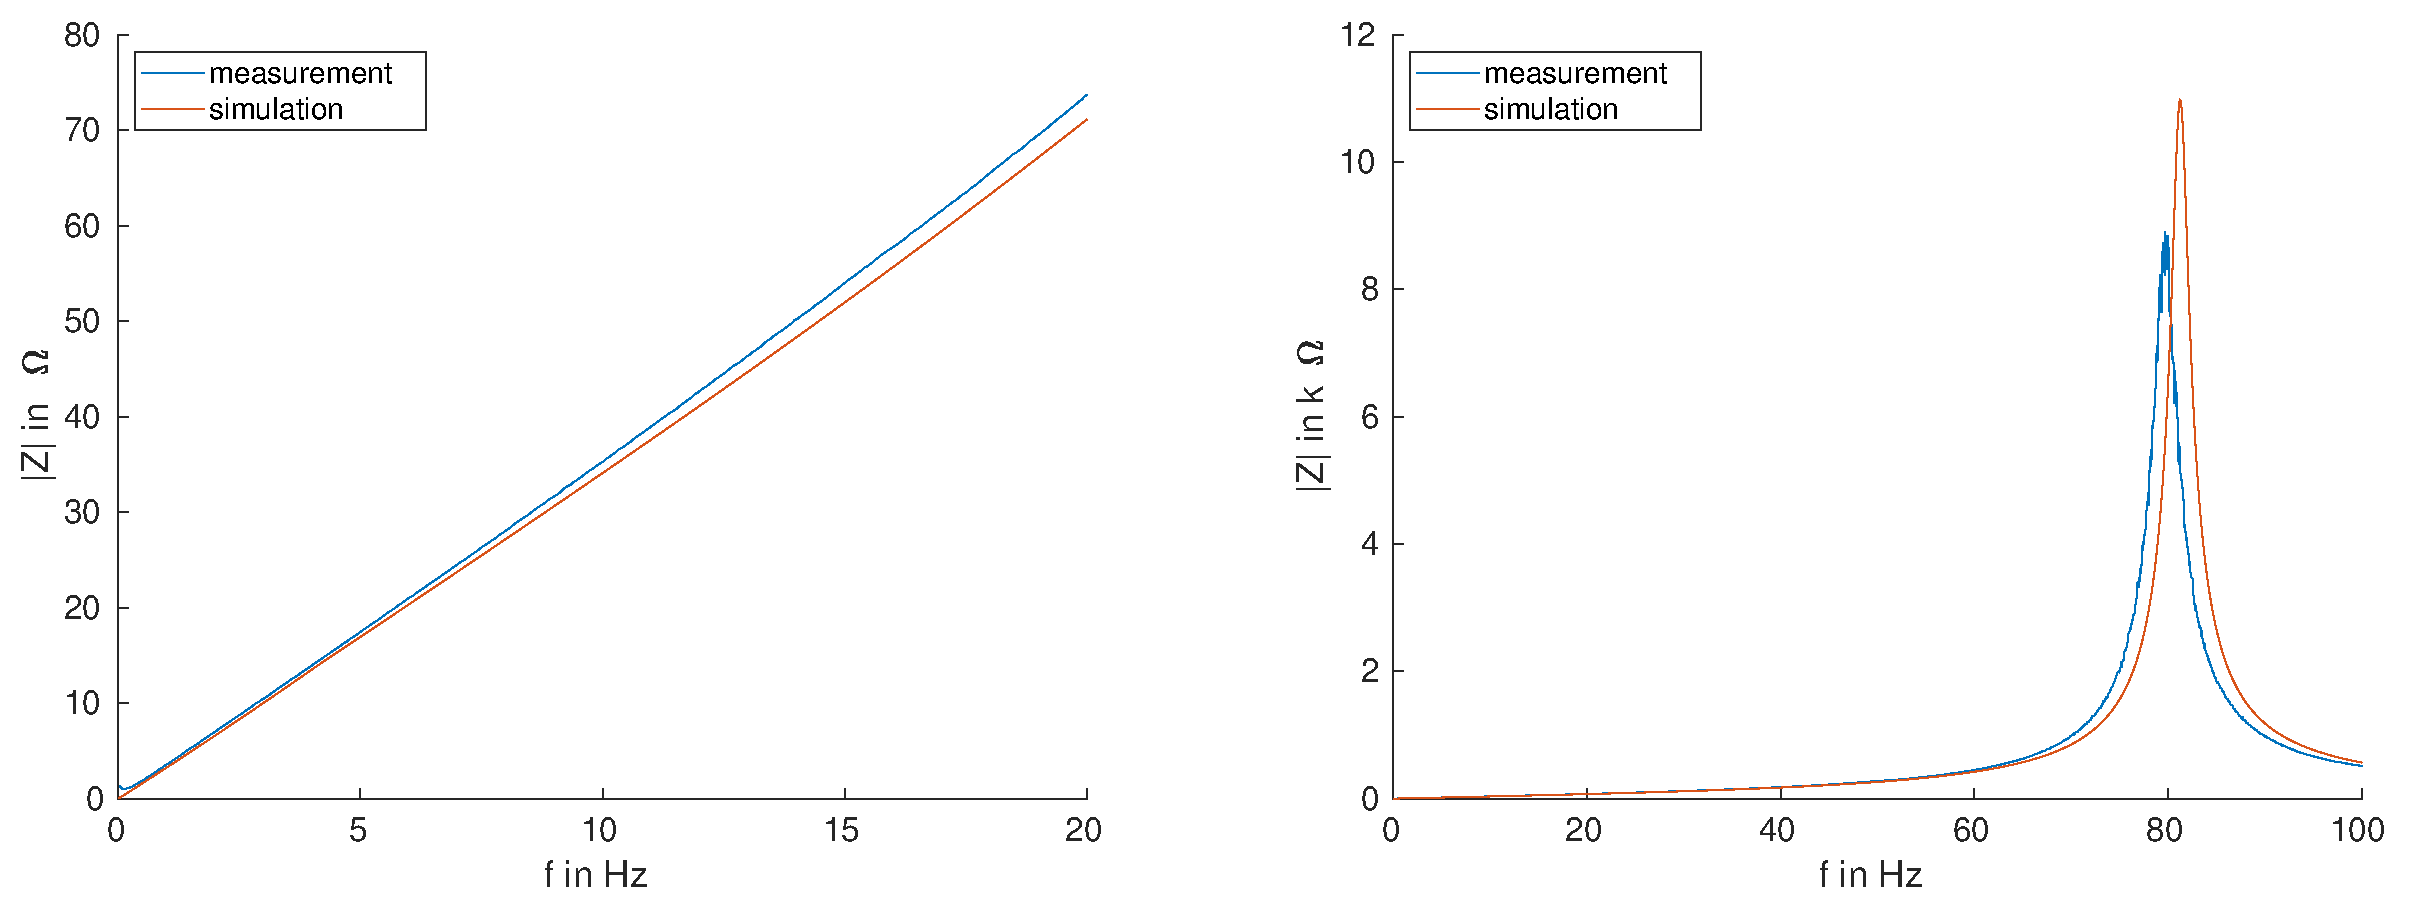
\includegraphics[width=\textwidth]{Z_ges_7KS_SimMeas}
	\caption{Gegen\"uberstellung der gemessenen, mit der simulierten Ringkernimpedanz f\"ur eine Anzahl von sieben Kurzschl\"ussen}
	\label{fig:boxpolycrossrk7ks}
\end{figure}

Eine m\"ogliche Erkl\"arung daf\"ur w\"are, dass die simulierten Kurzschl\"usse idealere Materialeigenschaften, bessere Kontaktierung sowie eine h\"ohere Formsicherheit aufweisen, als es das Kupfer und die Verschraubung in der Realit\"at liefern k\"onnen. Die Gegen\"uberstellung aller Kurzschlussanordnungen in Simulation und Messung sind in Anhang~\ref{sec:simmesskomplett} abgebildet.


\section{Auswertung der Kurzschlussanordnungen}
Nachdem die Messungen, sowie die Simulationen gegeneinander abgeglichen sind, kann die Auswertung der Kurzschlussversuche begonnen werden. Dazu wird nur die reine Ringkernimpedanz betrachtet und nach der Beschreibung in Kapitel~\ref{chap:simulation} berechnet. Analog zum in Abschnitt~\ref{sec:ringkern} beschriebenen Vorgehen, wird auch hierzu die Impedanz $Z_{rk}$ aus der gemessenen Impedanz $Z_{ges}$ nach Gleichung~\ref{eq:Zrk} herausgerechnet. Somit l\"asst sich isoliert betrachten, wie viel Anteil der Ringkernimpedanz durch das Hinzuf\"ugen der Kurzschl\"usse noch verbleibt. Dazu  werden die in Unterkapitel~\ref{sec:shorts} angef\"uhrten Variationsparameter gegenübergestellt.
\par
Für die Auswertung werden die Impedanzmesswerte in Relation zur Impedanz der Testbox ohne Kurzschlüsse gesetzt. Die prozentuale Abweichung kann dann wie folgt berechnet und für verschiedene Variationen verglichen werden.
\begin{equation}
	a_{Prozentual}(f) = \frac{Z_{rk}(f) - Z_{var}(f)}{Z_{rk}(f)}\cdot 100 = \left(1-\frac{Z_{var}(f)}{Z_{rk}(f)}\right)\cdot 100
	\label{eq:maxdiffpercent}
\end{equation}
In der folgenden Ausführung wird für $Z_{var}$ die Impedanz des zu betrachtenden Parameters eingesetzt. $Z_{rk}$ bezeichnet die Impedanz des Ringkerns ohne Kurzschl\"usse.

\subsection{Anzahl der Kurzschl\"usse}
Um den Einfluss verschiedener Anzahlen an Kurzschl\"ussen zu analysieren, werden ein bis acht identische Kurzschl\"usse in der Testbox montiert. Abbildung~\ref{fig:ringcorenumberCST} zeigt die Positionen der montierten Kurzschl\"usse.

\begin{figure}[htb]
	\centering
	\subfloat{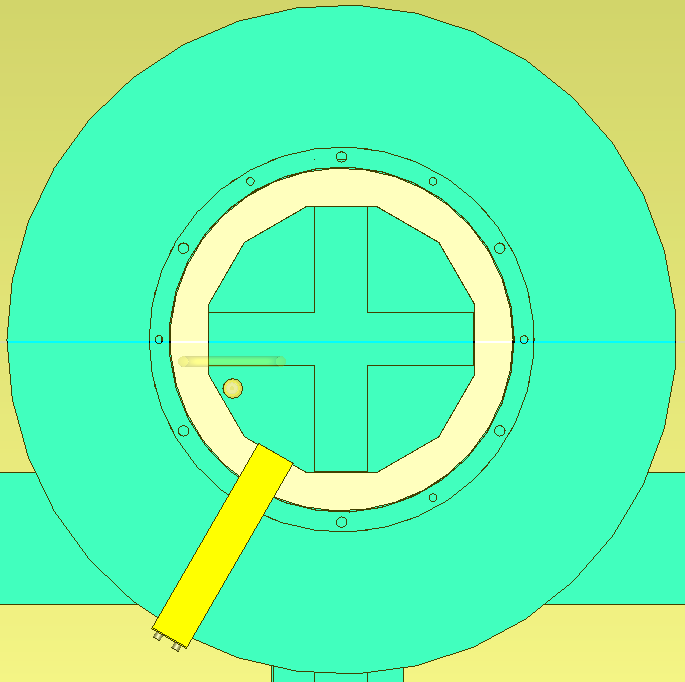
\includegraphics[height=0.24\textwidth]{1ksb30}}
	\hspace{0.0065\textwidth}
	\subfloat{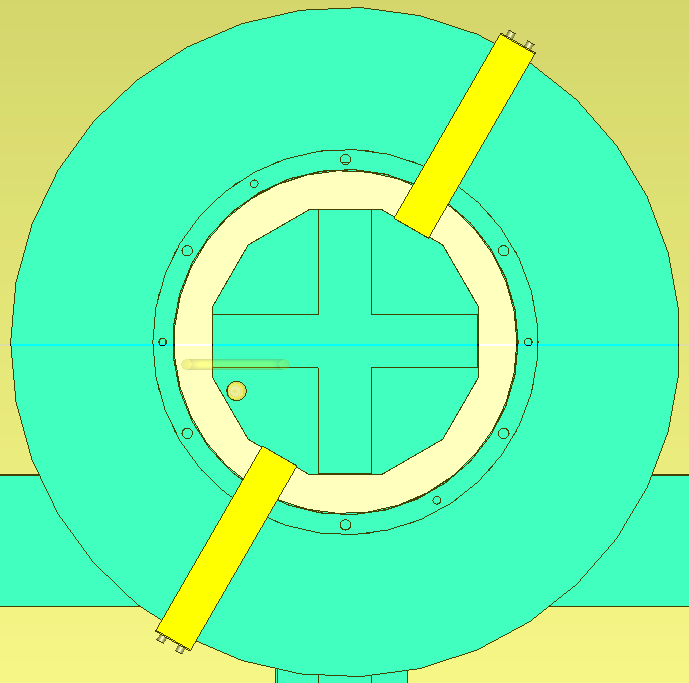
\includegraphics[height=0.24\textwidth]{2ksb30}}
	\hspace{0.0065\textwidth}
	\subfloat{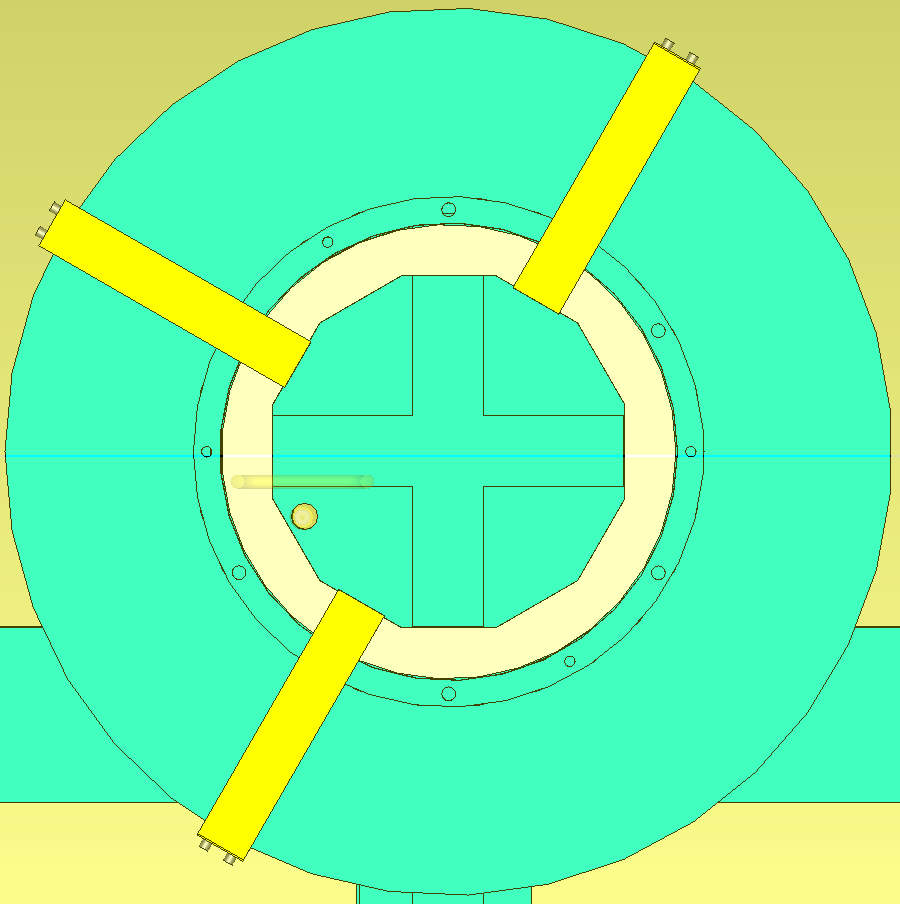
\includegraphics[height=0.24\textwidth]{3ksb30}}
	\hspace{0.0065\textwidth}
	\subfloat{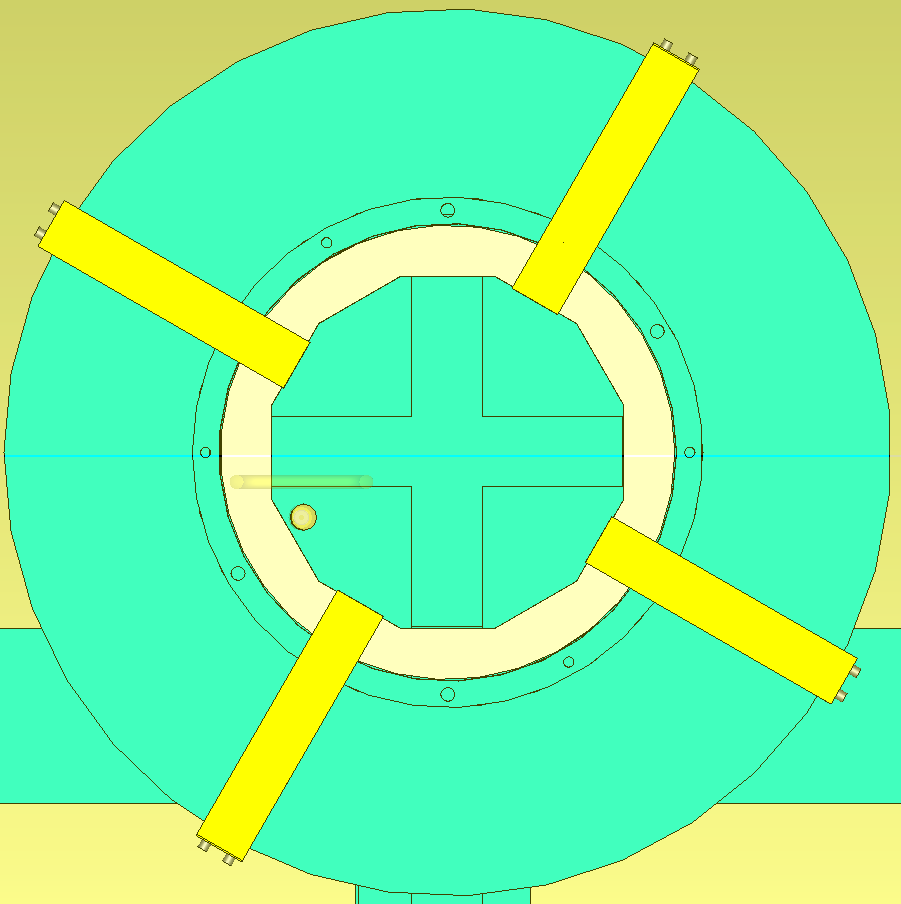
\includegraphics[height=0.24\textwidth]{4ksb30}}
	\\
	\subfloat{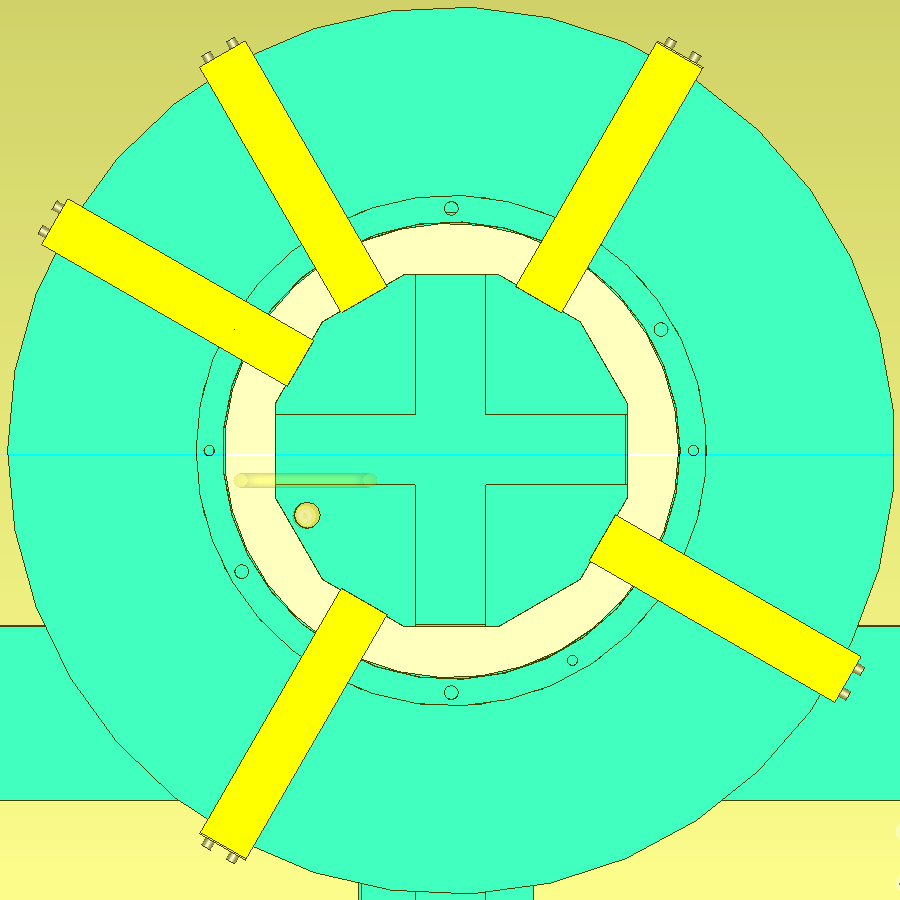
\includegraphics[height=0.24\textwidth]{5ksb30}}
	\hspace{0.0065\textwidth}
	\subfloat{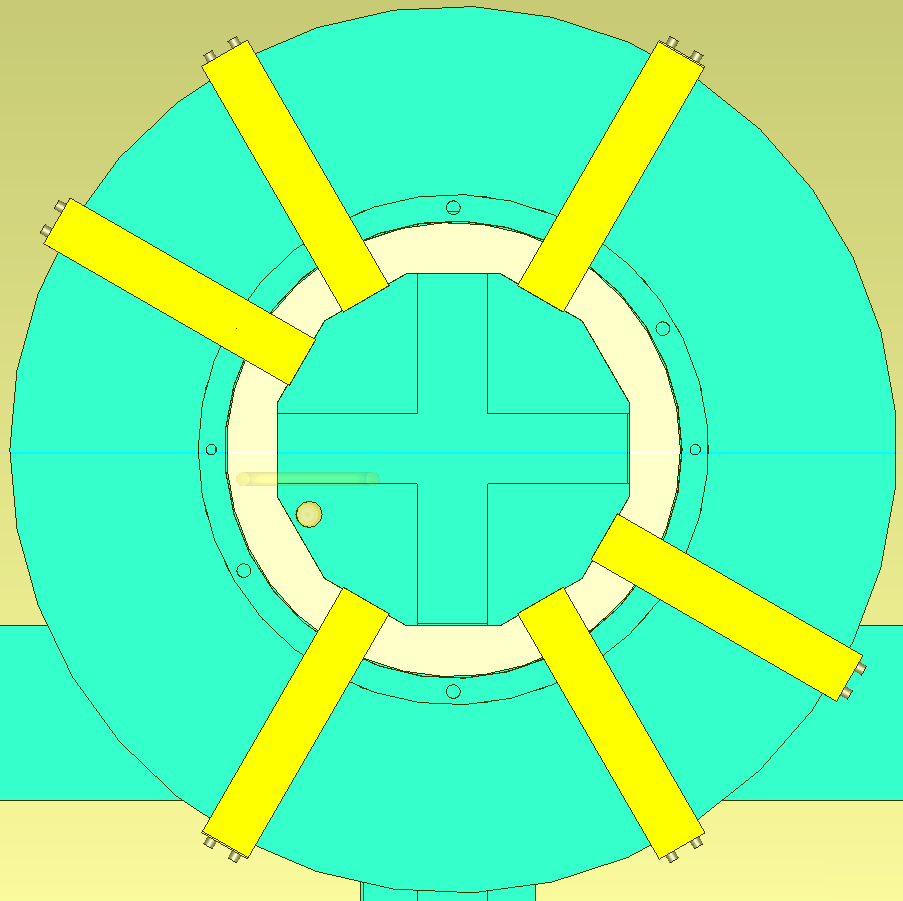
\includegraphics[height=0.24\textwidth]{6ksb30}}
	\hspace{0.0065\textwidth}
	\subfloat{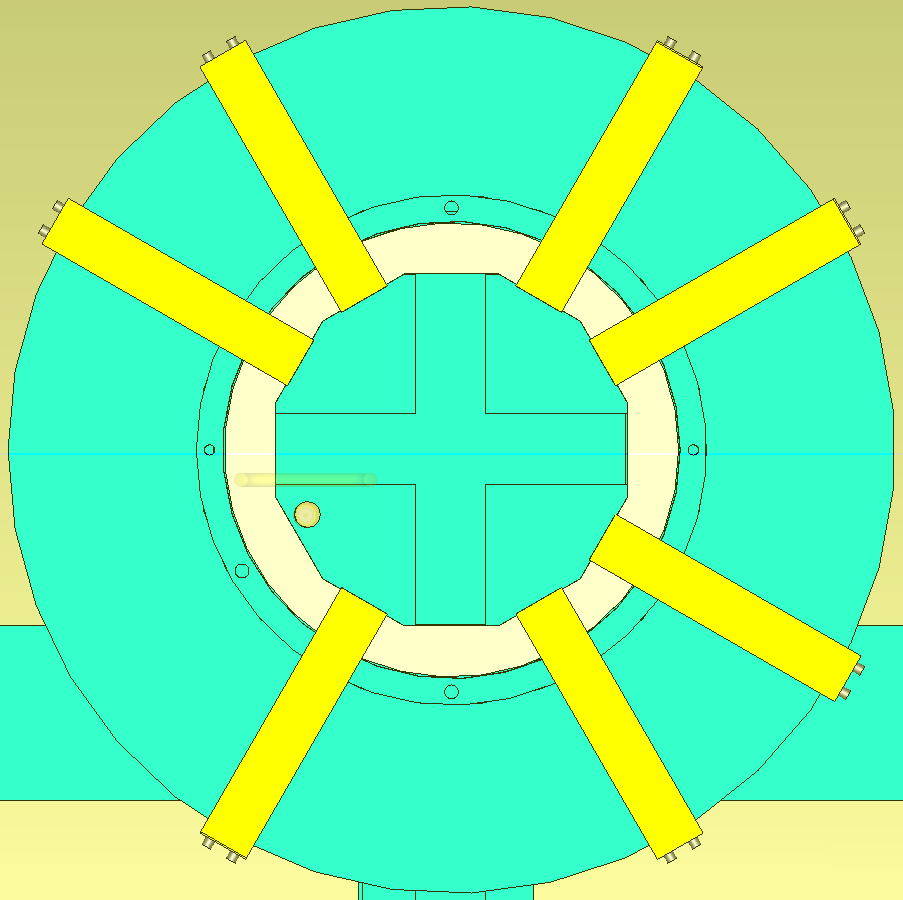
\includegraphics[height=0.24\textwidth]{7ksb30}}
	\hspace{0.0065\textwidth}
	\subfloat{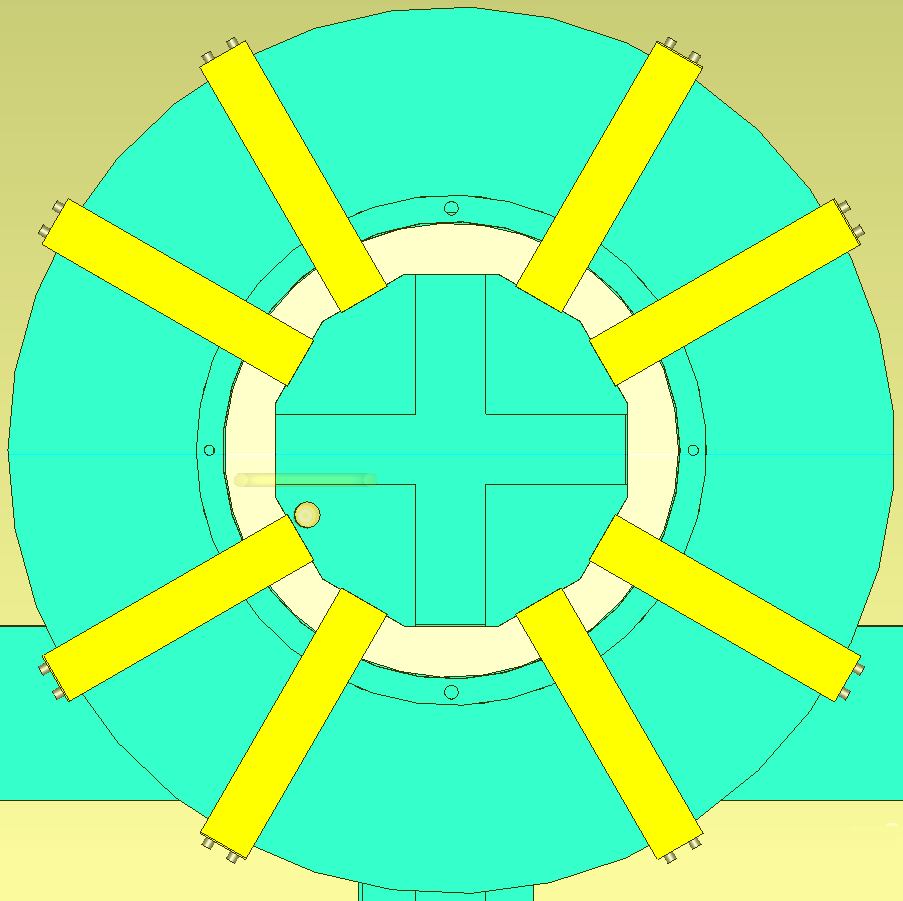
\includegraphics[height=0.24\textwidth]{8ksb30}}
	\caption{Unterschiedliche Anzahlen an montierten Kurzschl\"ussen an verschiedenen Positionen.}
	\label{fig:ringcorenumberCST}
\end{figure}

% \todo[inline,color=red!30]{Erkl\"aren warum 8KS bei der Auswertung nicht mehr auftaucht}  
Die achte Kurzschlusschiene, welche in Grafik~\ref{fig:ringcorenumberCST} zu sehen ist, konnte bei der endg\"ultigen Auswertung nicht ber\"ucksichtigt werden. Dieser Kurzschluss liegt sehr nah am Einkopplungsrohr, sodass ein direkter Kontakt dazu besteht. F\"ugt man einen Abstandshalter aus Schaumstoff zu, so wird die Einkopplung etwas nach oben gebogen. Die Messung liefert daher verf\"alschte Ergebnisse, welche deutlich st\"arker von der Simulation abweichen, als bei anderen Messungen. Auch dieses Verhalten ist in Anhang~\ref{sec:simmesskomplett} abgebildet. F\"ur die endg\"ultige Auswertung wurden folglich nur ein bis sieben Kurzschl\"usse betrachtet. Die resultierende Ringkernimpedanz f\"ur die einzelnen Kurzschlussanordnungen ist in Abbildung~\ref{fig:ringcorenumber} \"uber der Frequenz aufgetragen.


\newpage

\begin{figure}[htb]
	\centering
	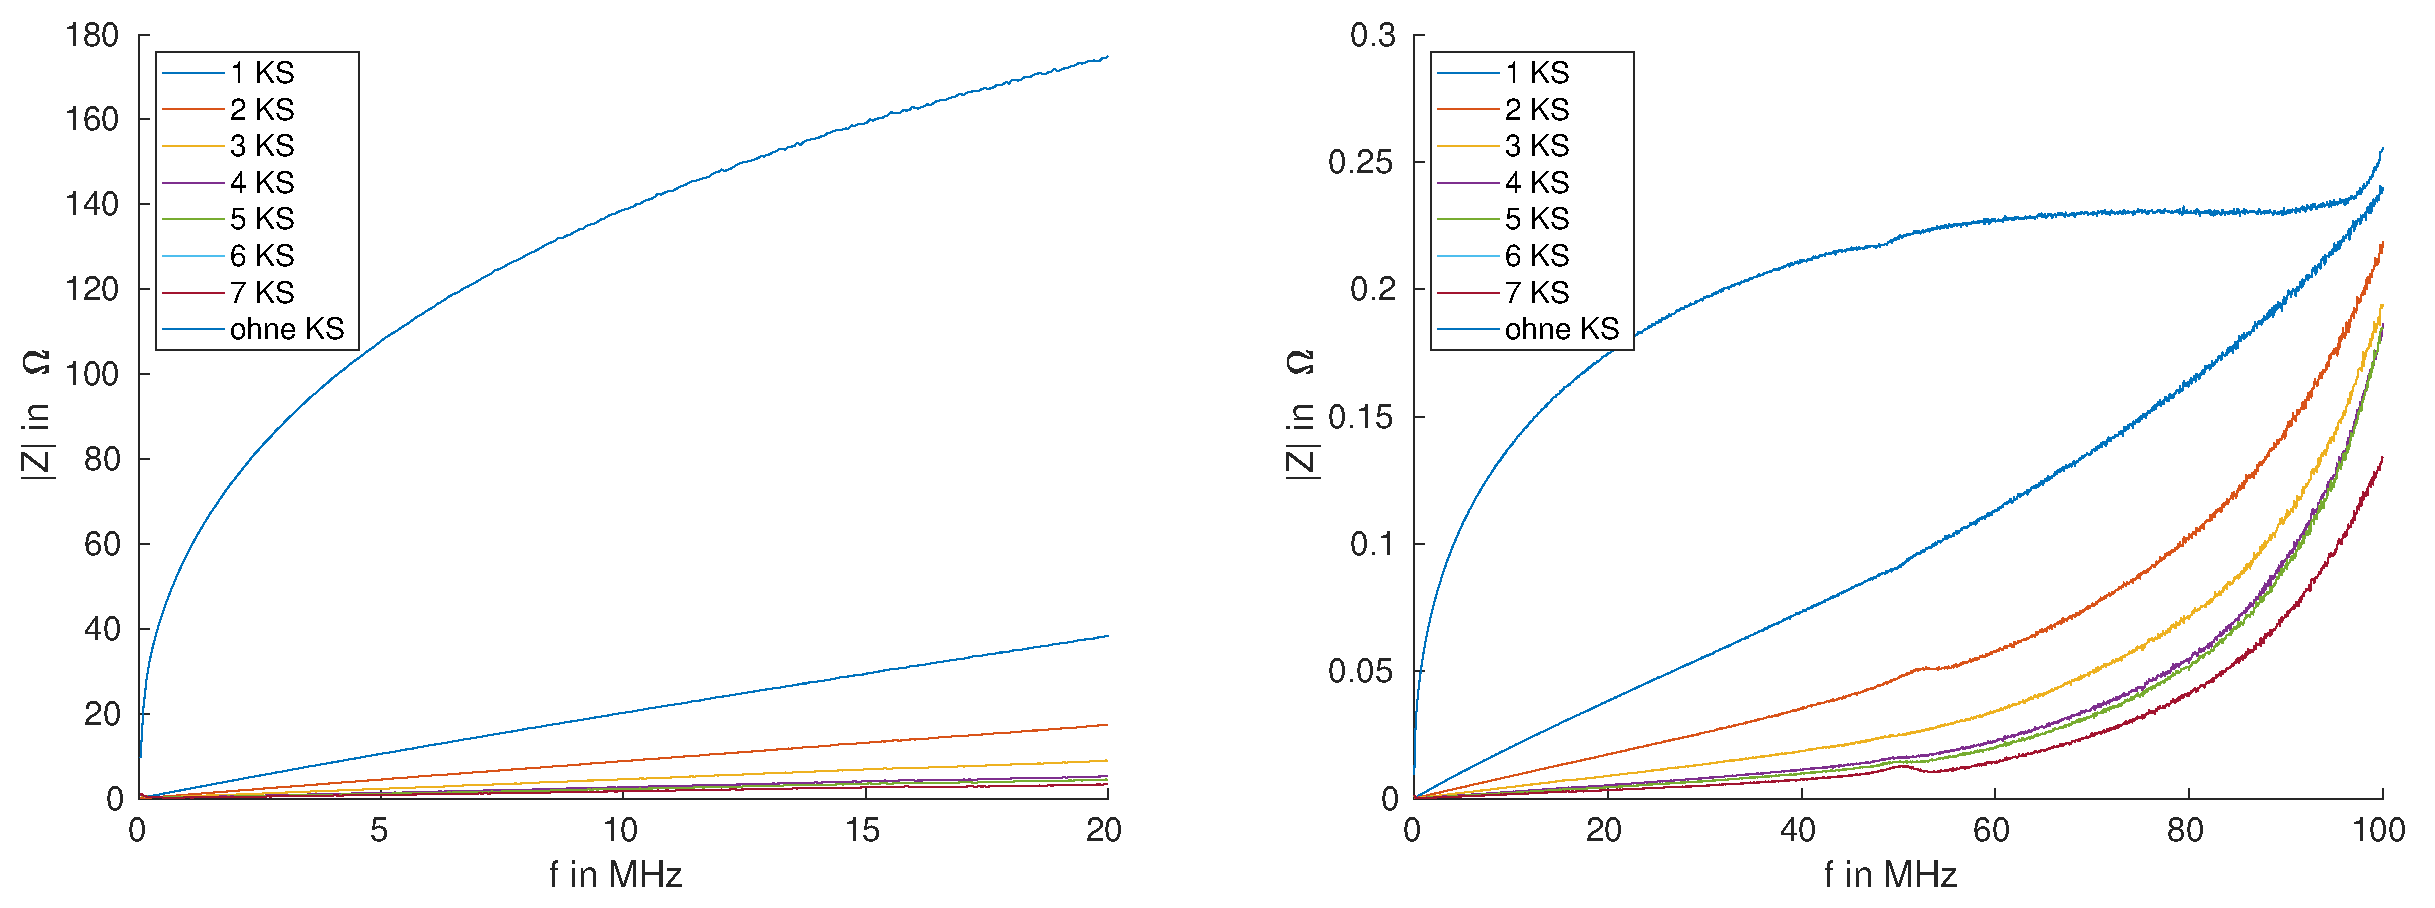
\includegraphics[width=\textwidth]{impedance_numberKS_ringcore}
	\caption{Gegen\"uberstellung der Ringkernimpedanz \"uber der Frequenz f\"ur verschiedene Anzahlen an Kurzschl\"ussen}
	\label{fig:ringcorenumber}
\end{figure}

Es f\"allt auf, dass der gr\"o\ss{}te Unterschied zwischen dem Ringkern ohne Kurzschluss und einem Kurzschluss besteht. Das bedeutet, dass die Montage weiterer Kurzschl\"usse mit zunehmender Anzahl weniger effektiv ist. Dies wird durch die folgenden Betrachtung verdeutlicht, bei die Impedanz an festen Frequenzen ausgewertet und \"uber der Anzahl an Kurzschl\"ussen aufgetragen wird. Dies geschieht bei 5, 10 und $\SI{20}{\mega\hertz}$, da insbesondere der niedrigere Frequenzbereich f\"ur den Beschleunigerbetrieb von Relevanz ist~\citep{frey2015status}. Die Gegen\"uberstellung ist in Abbildung~\ref{fig:ringcorenumber20} aufgetragen.

\begin{figure}[htb]
	\centering
	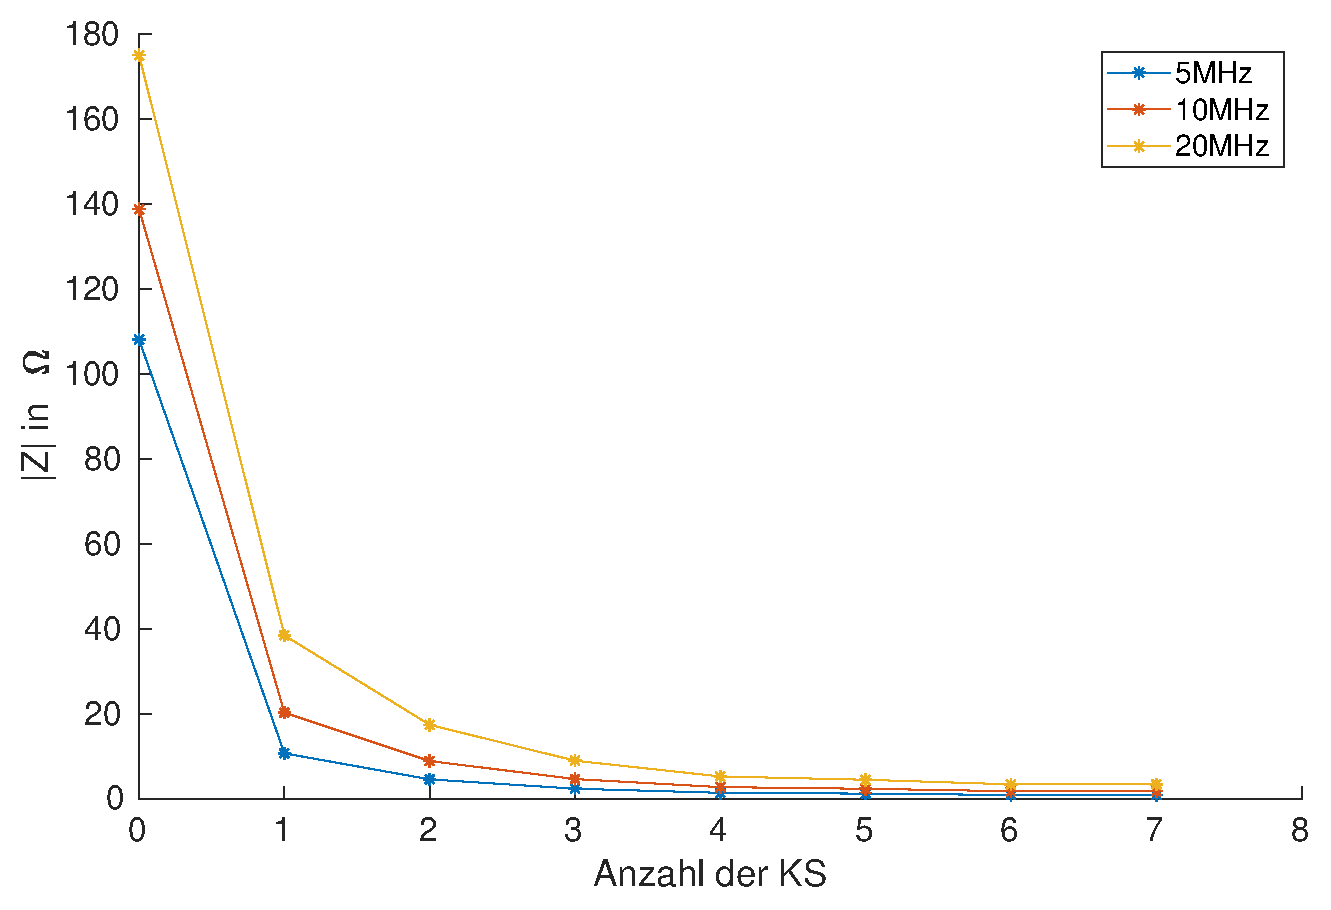
\includegraphics[width=0.5\textwidth]{RK_Impedanz_numberKS_frequenz}
	\caption{Gegen\"uberstellung der Ringkernimpedanz mit verschiedenen Anzahlen an Kurzschl\"ussen bei 5, 10 und $\SI{20}{\mega\hertz}$.}
	\label{fig:ringcorenumber20}
\end{figure}

Wird die Impedanz mit Kurzschlüssen in Relation zur Ringkernimpedanz gesetzt, kann der Effekt der Kurzschl\"usse wie beschrieben dargestellt werden. Für einen Kurzschluss ergibt sich bei \SI{20}{\mega\hertz} somit eine prozentuale Verringerung von 
\begin{equation}
	\frac{\SI{175,1145}{\Omega} - \SI{38,4525}{\Omega}}{\SI{175,1145}{\Omega}}\cdot 100 = \SI{78,042}{\%}.
	\label{eq:maxdiffpercentzeroone}
\end{equation}
Für zwei Kurzschlüsse errechnet nach Formel~\ref{eq:maxdiffpercent} sich eine prozentuale Abweichung von $\SI{90,08}{\%}$, was gegenüber einem Kurzschluss eine weitere Verringerung um $\SI{12,038}{\%}$ bedeutet. Diese weitere Verringerung fällt damit deutlich geringer aus, als es bereits durch einen Kurzschluss der Fall ist. Auch der Vergleich von einem zu sieben Kurzschlüssen, die eine Verringerung der Ringkernimpedanz von $\SI{98,09}{\%}$ hervorrufen, fällt mit weiteren $\SI{20,048}{\%}$ vergleichsweise gering aus.

\subsection{Breite der Kurzschl\"usse}
Die Breite der Kurzschl\"usse ist ein Parameter, welcher durch die schienenartige Form der Kurzschl\"usse leicht zu variieren ist, da diese nur aus einem Blech geschnitten werden. Die montierten Kurzschl\"usse verschiedener Breiten sind in Abbildung~\ref{fig:ringcorewidthCST} abgebildet.

\begin{figure}[htb]
	\centering.
	\subfloat[$\SI{20}{\milli\meter}$]{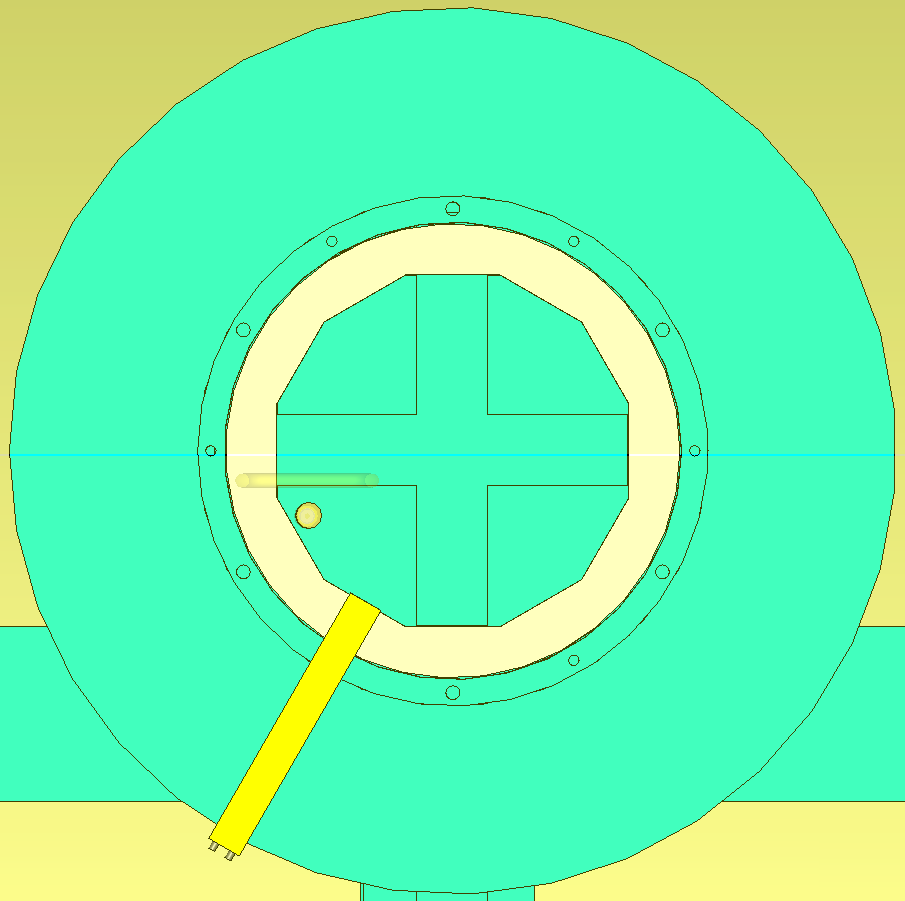
\includegraphics[height=0.3\textwidth]{1ksb20}}
	\hspace{0.02\textwidth}
	\subfloat[$\SI{30}{\milli\meter}$]{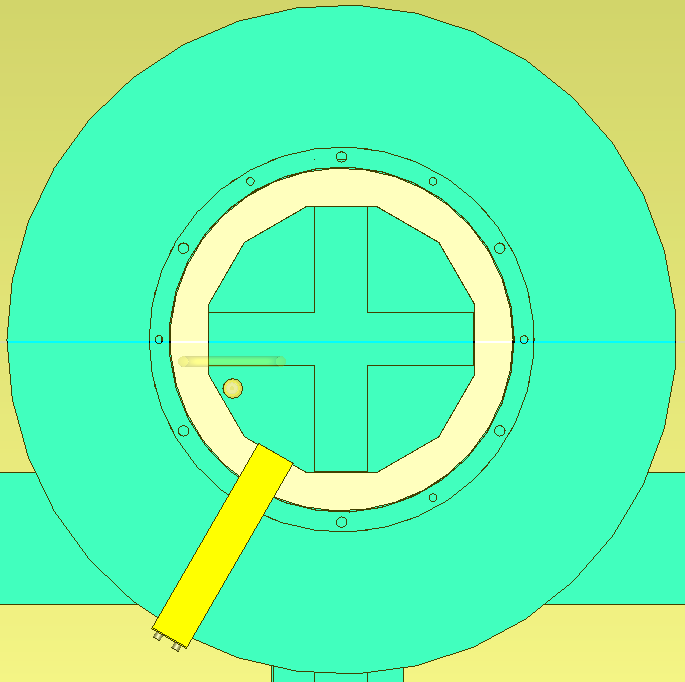
\includegraphics[height=0.3\textwidth]{1ksb30}}
	\hspace{0.02\textwidth}
	\subfloat[$\SI{50}{\milli\meter}$]{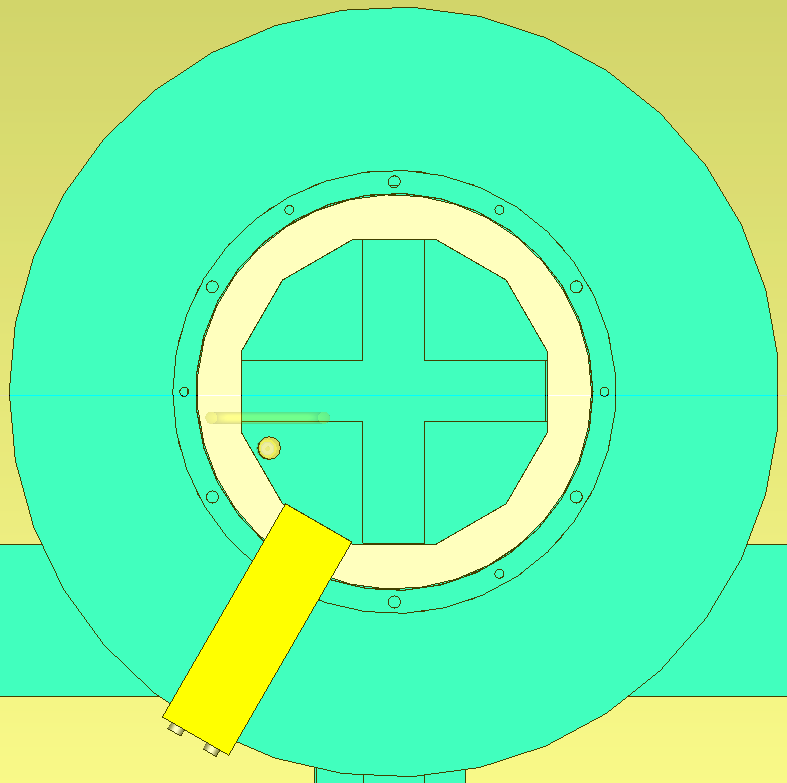
\includegraphics[height=0.3\textwidth]{1ksb50}}
	\caption{Jeweils ein montierter Kurzschluss mit verschiedenen Breiten.}
	\label{fig:ringcorewidthCST}
\end{figure}



\newpage



Da eine h\"ohere Anzahl an Kurzschl\"ussen eine verringerte Ringkernimpedanz als Ergebnis liefert, liegt die Vermutung nahe, dass auch breitere Kurzschl\"usse die Ringkernimpedanz weiter verringern k\"onnen. Die Gegen\"uberstellung der Ringkernimpedanz $Z_{rk}$ ist in Abbildung~\ref{fig:ringcorewidth} zu sehen.

\begin{figure}[htb]
	\centering
	\subfloat[1 Kurzschluss]{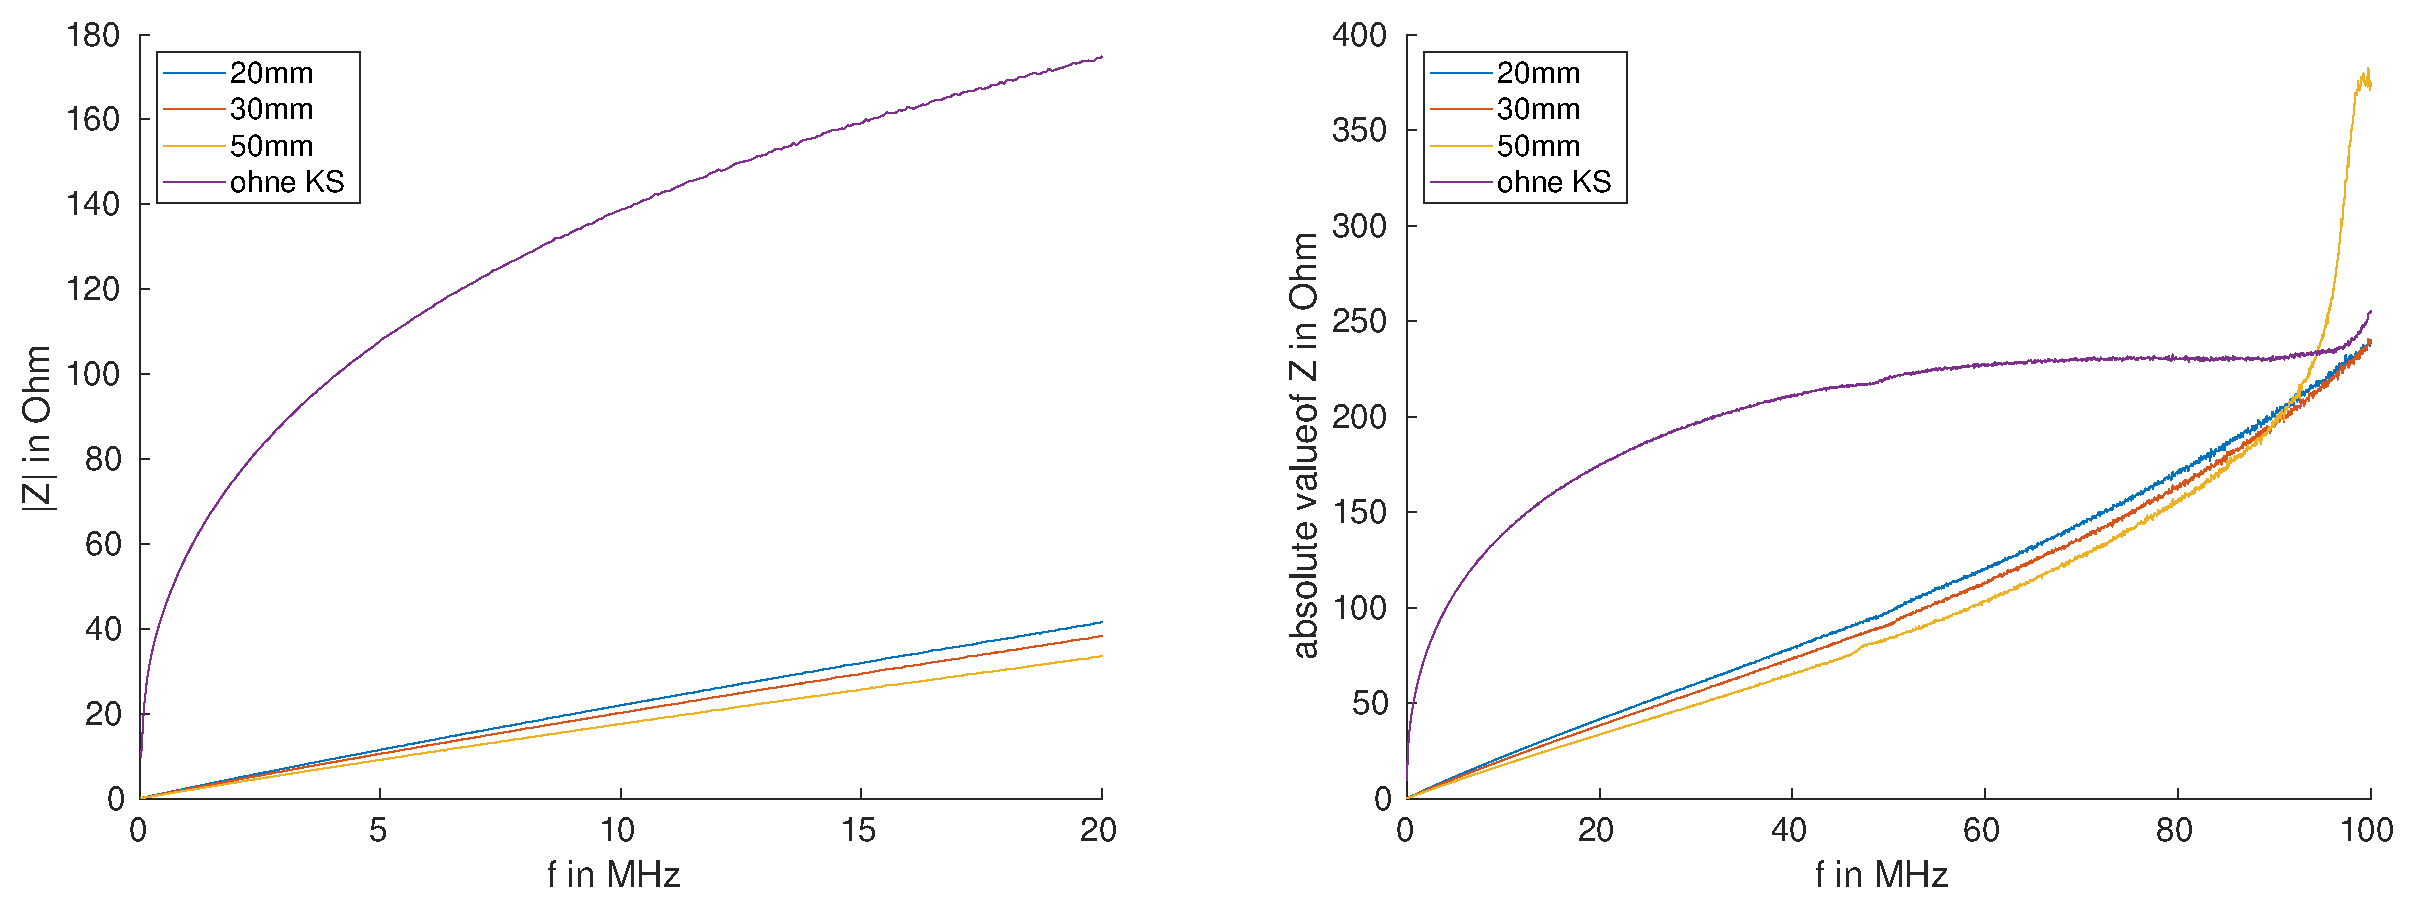
\includegraphics[width=\textwidth]{Z_RK_width_1KS}}
	\\
	\subfloat[2 Kurzschl\"usse]{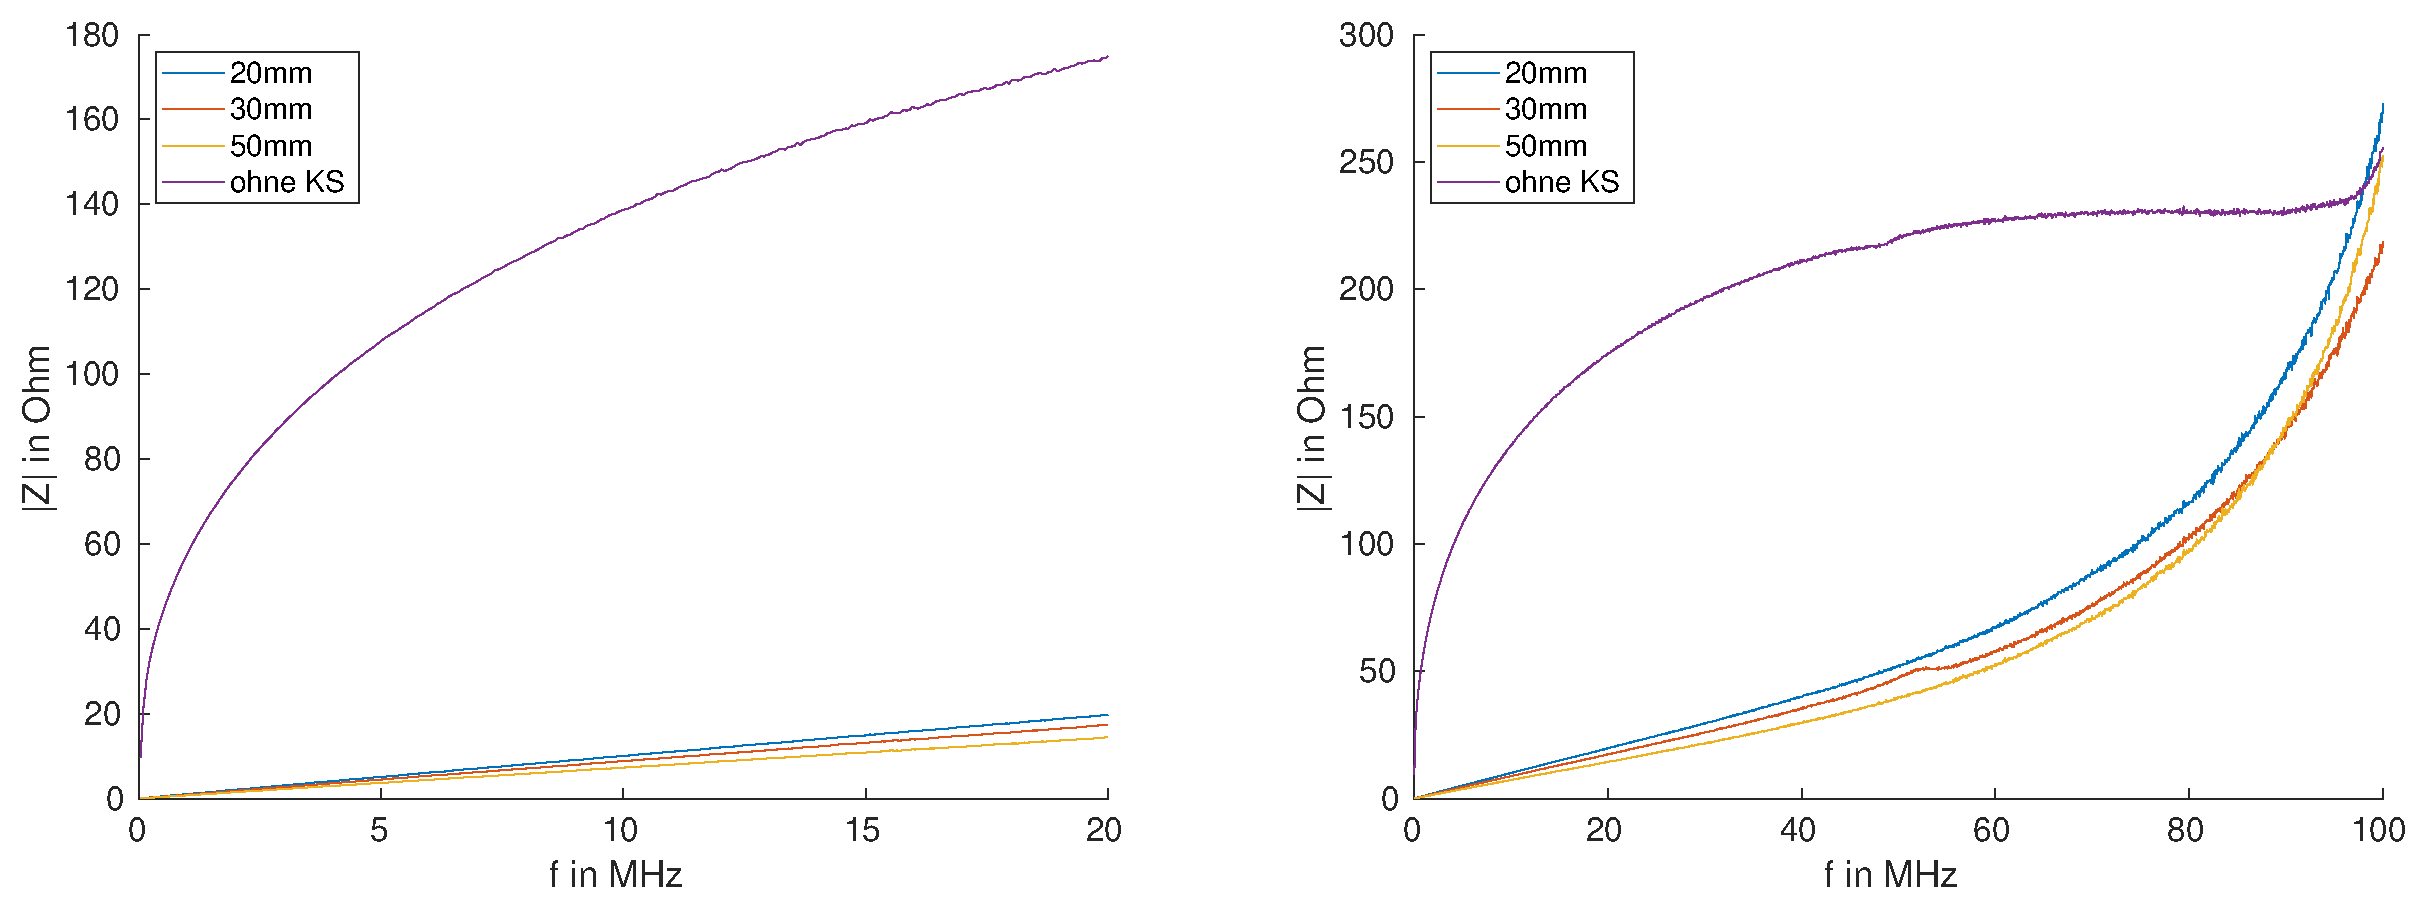
\includegraphics[width=\textwidth]{Z_RK_width_2KS}}
	\caption{Gegen\"uberstellung der Ringkernimpedanz f\"ur verschiedene Breiten der Kurzschl\"usse.}
	\label{fig:ringcorewidth}
\end{figure}

Auch hier wird wieder ein genaueres Augenmerk auf den relevanten Frequenzbereich unterhalb von $\SI{20}{\mega\hertz}$ gelegt. Dazu wird die Impedanz wieder bei den Frequenzen 5, 10 und $\SI{20}{\mega\hertz}$ dargestellt und die verschiedenen Breiten gegen\"ubergestellt. Dies ist in Abbildung~\ref{fig:ringcorewidth20} gezeigt.



\newpage



\begin{figure}[h]
	\centering
	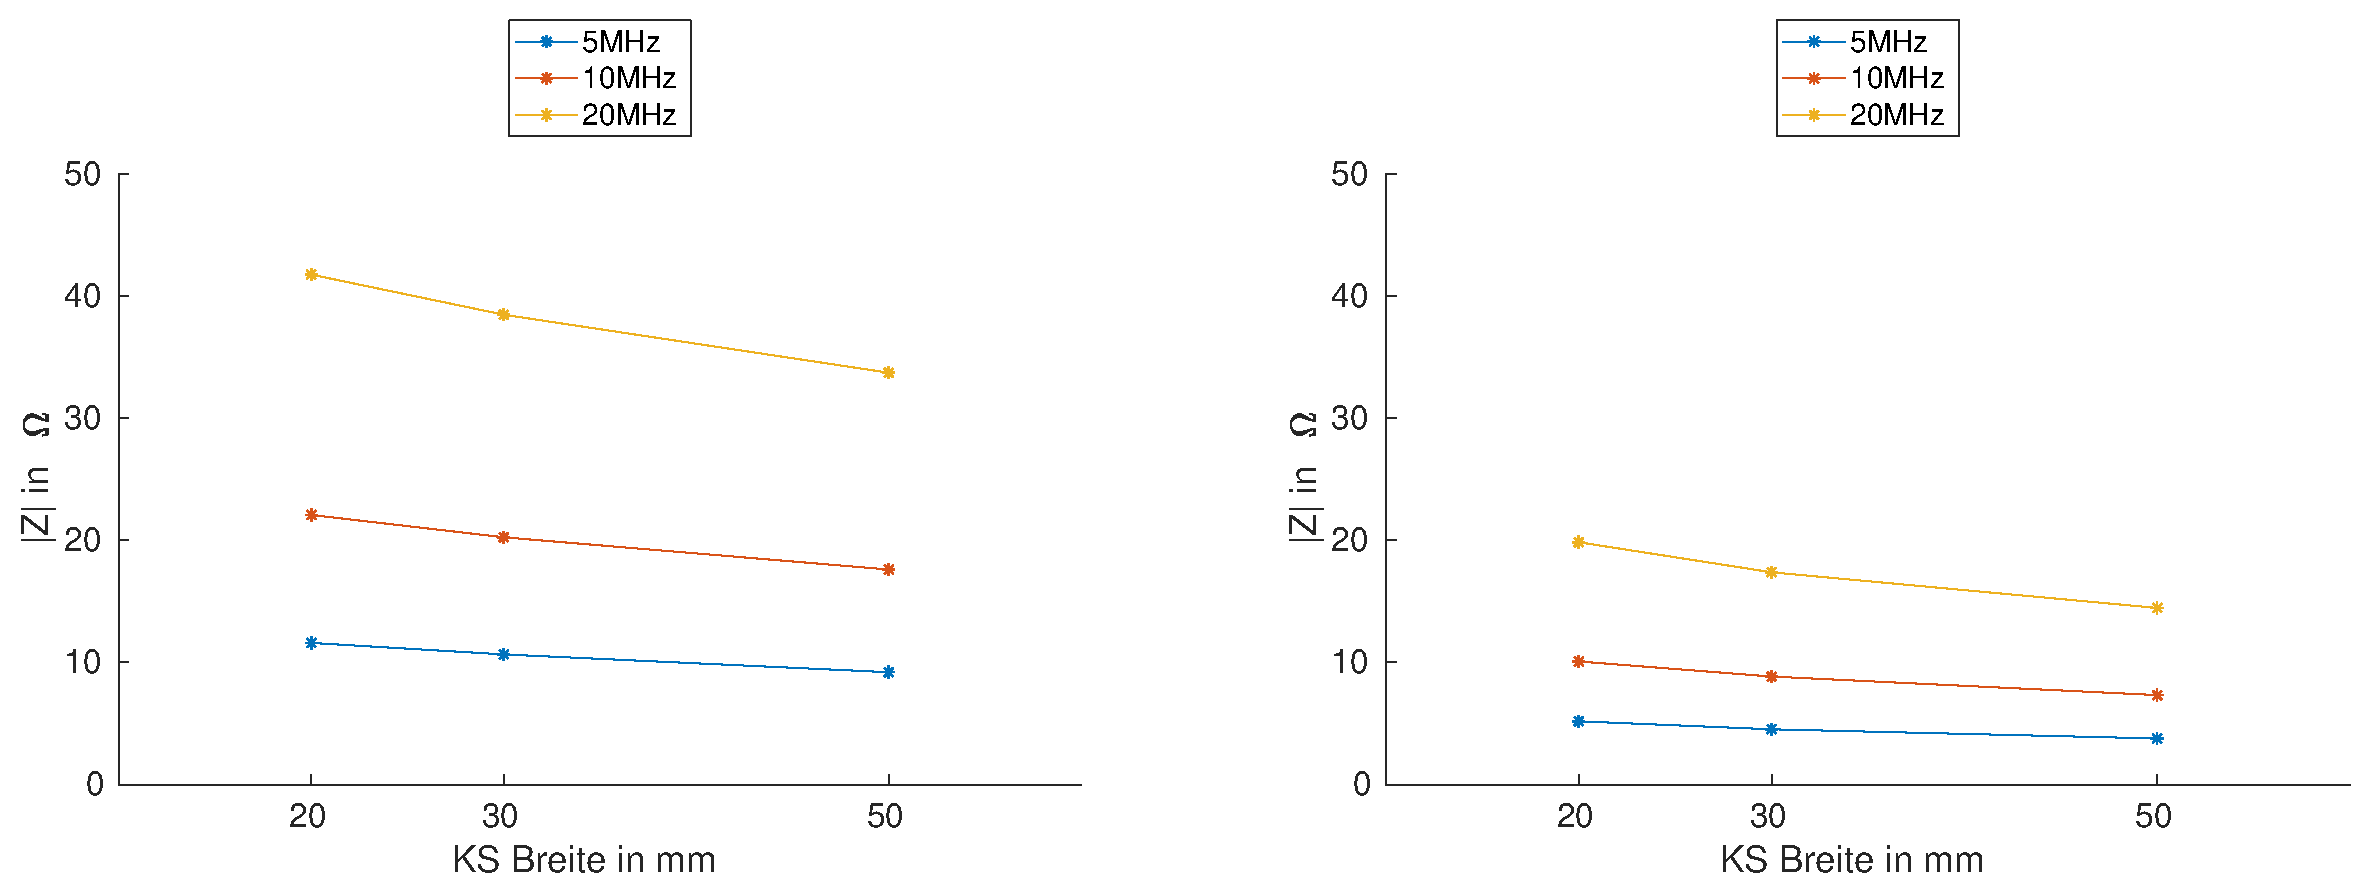
\includegraphics[width=\textwidth]{RK_Impedanz_width_frequenz}
	\caption{Gegen\"uberstellung der Ringkernimpedanz bei 5, 10 und $\SI{20}{\mega\hertz}$. Links: 1KS, rechts: 2KS.}
	\label{fig:ringcorewidth20}
\end{figure}

Das Ergebnis zeigt, dass ein breiterer Kurzschluss das Ergebnis der resultierenden Ringkernimpedanz weiter verringert. Diese Variation liefert im Extremfall, also dem Unterschied von $\SI{20}{\milli\meter}$ zu $\SI{50}{\milli\meter}$ bei einer Anzahl von zwei Kurzschl\"ussen und einer Frequenz von $\SI{20}{\mega\hertz}$, eine Verringerung der Ringkernimpedanz von rund $\SI{2,8}{\%}$. Dies zeigt, dass die Breite der Kurzschl\"usse eine geringere Auswirkung auf die resultierende Ringkernimpedanz hat, als die Anzahl der Kurzschl\"ussen. Besonders deutlich wird das im Vergleich zwischen einem Kurzschluss der Breite $\SI{50}{\milli\meter}$ mit zwei Kurzschl\"ussen der Breite $\SI{20}{\milli\meter}$ (siehe Anhang~\ref{anhang:Anordnung}). Trotz des geringeren Platzbedarfs, liefern die zwei schmalen Kurzschl\"usse eine deutlich geringere Impedanz.

\subsection{L\"ange der Kurzschl\"usse}
\"Ahnlich wie die Breite ist auch die L\"ange der Kurzschl\"usse problemlos zu varrieren. Hierbei ist allerdings darauf zu achten, dass die Kurzschlussb\"ugel mit Erh\"ohung der L\"ange auch n\"aher an den Rand der Testbox, beziehungsweise der Kavit\"at heran ragen. Die getesteten verschiedenen L\"angen sind in Abbildung~\ref{fig:ringcoreheightCST} gezeigt.

\begin{figure}[htb]
	\centering
	\subfloat[$\SI{160}{\milli\meter}$]{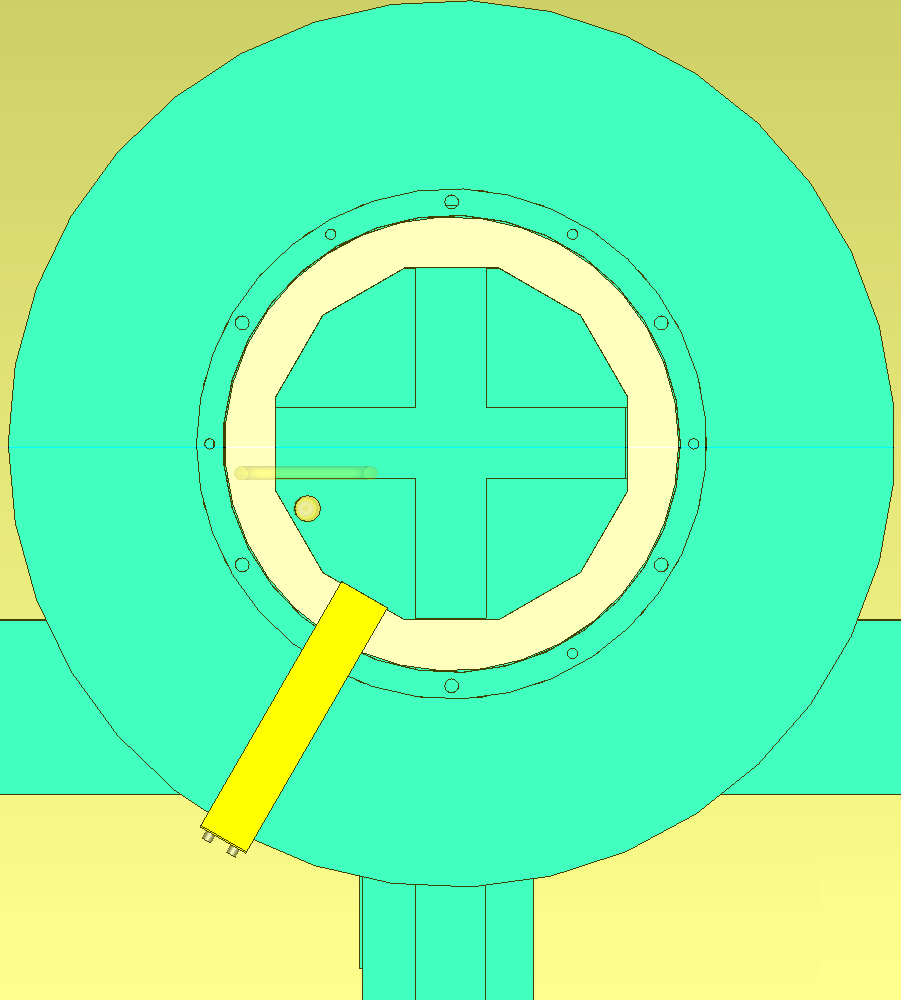
\includegraphics[height=0.3\textwidth]{1ksh160}}
	\hspace{0.05\textwidth}
	\subfloat[$\SI{200}{\milli\meter}$]{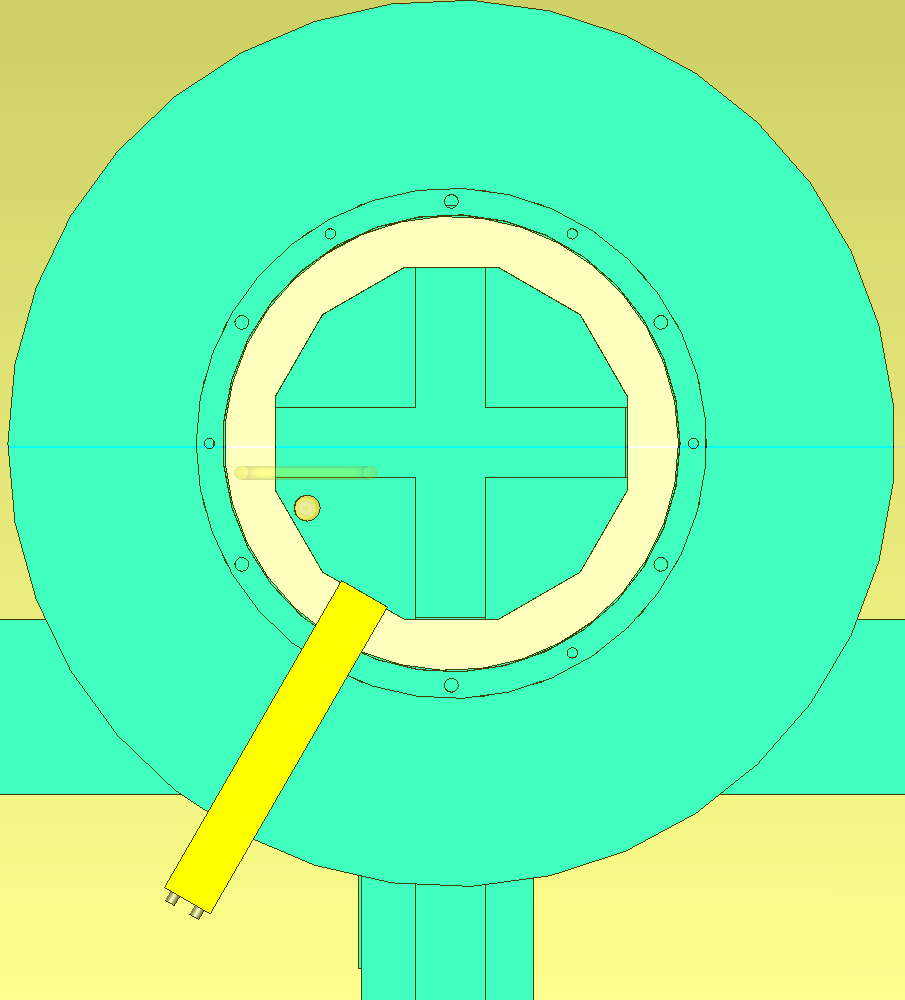
\includegraphics[height=0.3\textwidth]{1ksh200}}
	\hspace{0.05\textwidth}
	\subfloat[$\SI{250}{\milli\meter}$]{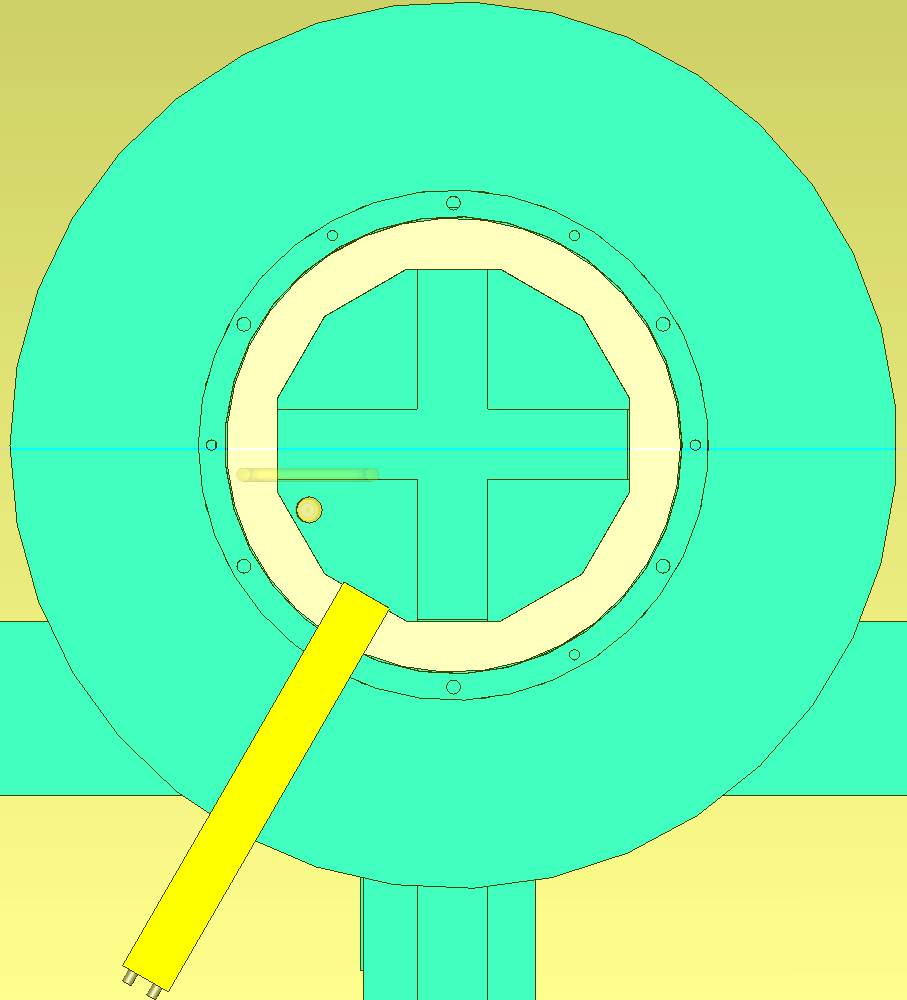
\includegraphics[height=0.3\textwidth]{1ksh250}}
	\caption{Jeweils ein montierter Kurzschluss mit verschiedenen L\"angen.}
	\label{fig:ringcoreheightCST}
\end{figure}

Die L\"ange der Kurzschl\"usse wird nach dem bekannten Vorgehen analysiert. Zun\"achst wird die Ringkernimpedanz \"uber der Frequenz nach Abbildung~\ref{fig:ringcoreheight} aufgetragen.

\begin{figure}[htb]
	\centering
	\subfloat[1 Kurzschluss]{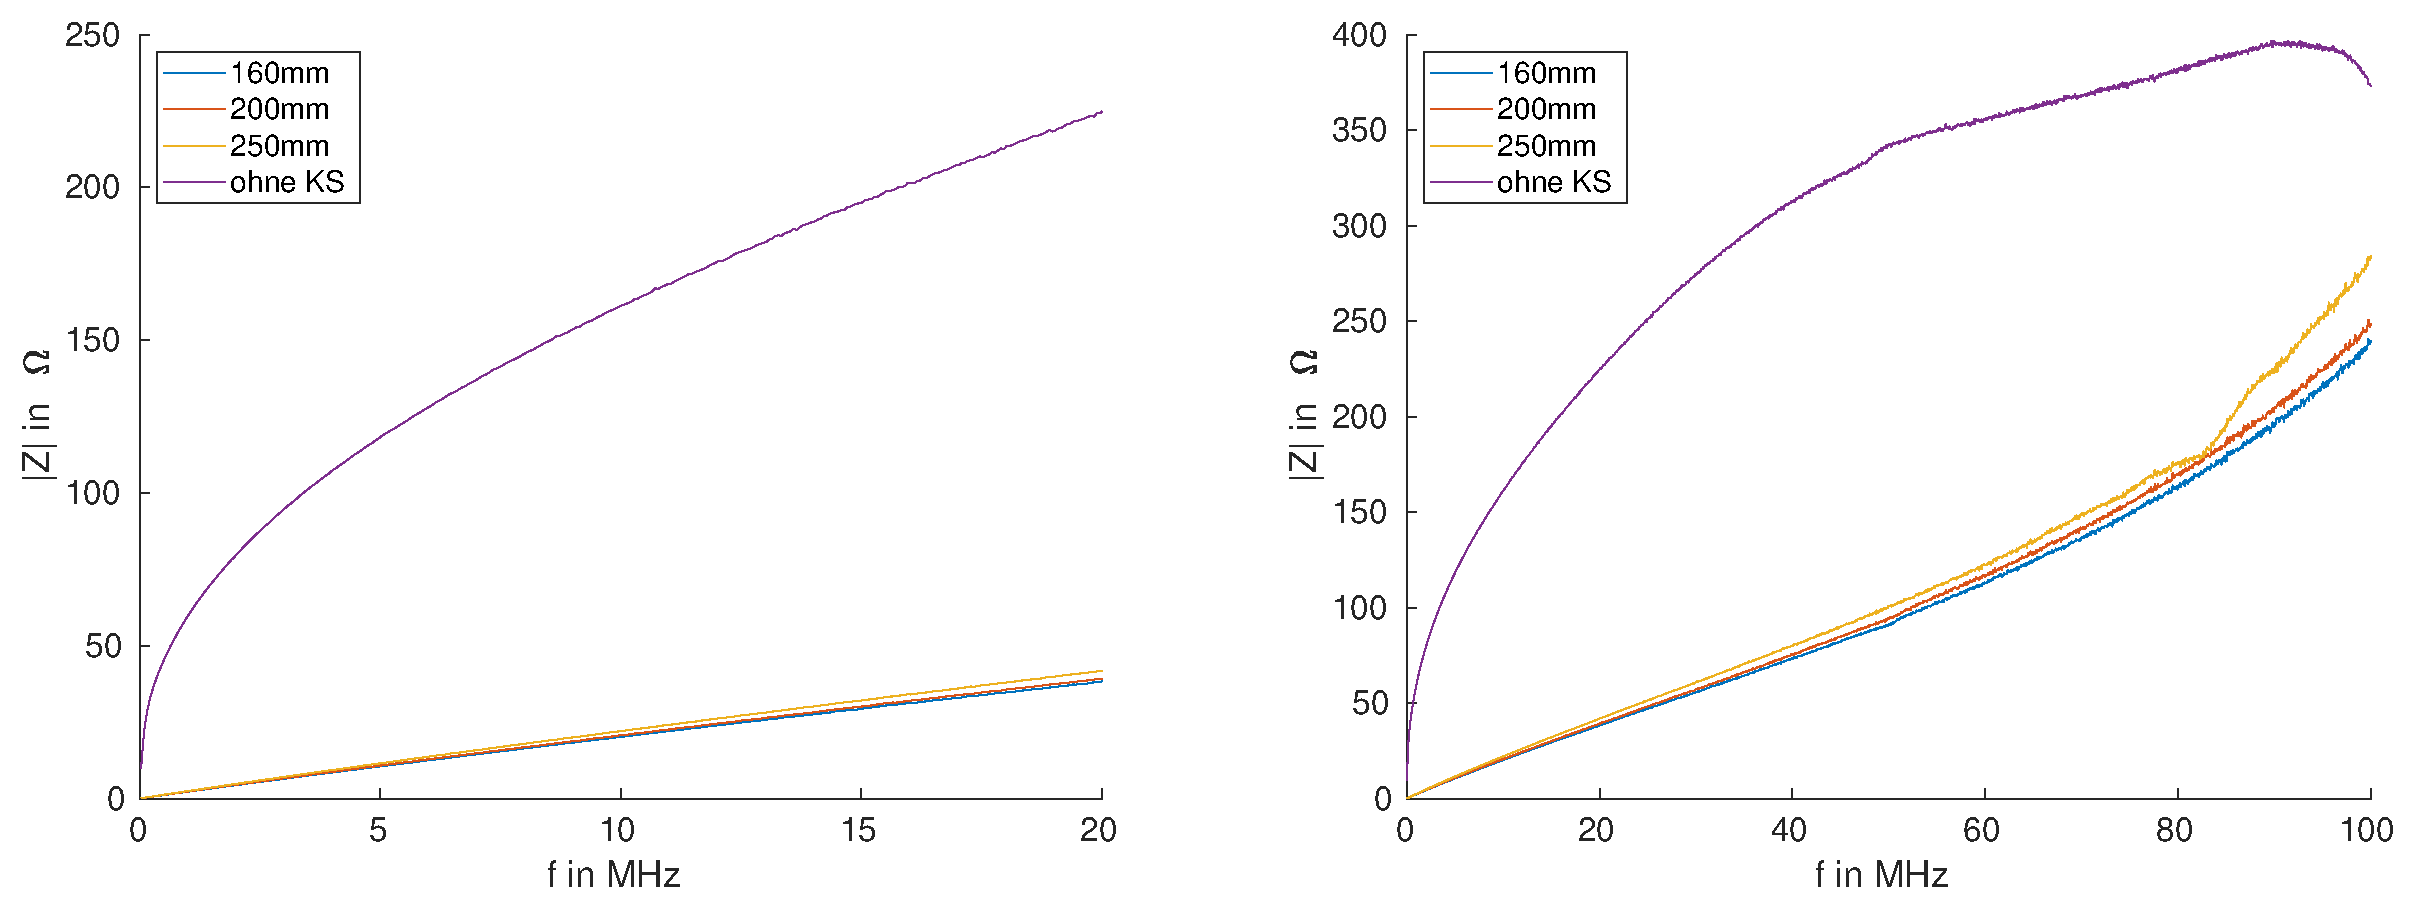
\includegraphics[width=\textwidth]{Z_RK_length_1KS}}
	\\
	\subfloat[2 Kurzschl\"usse]{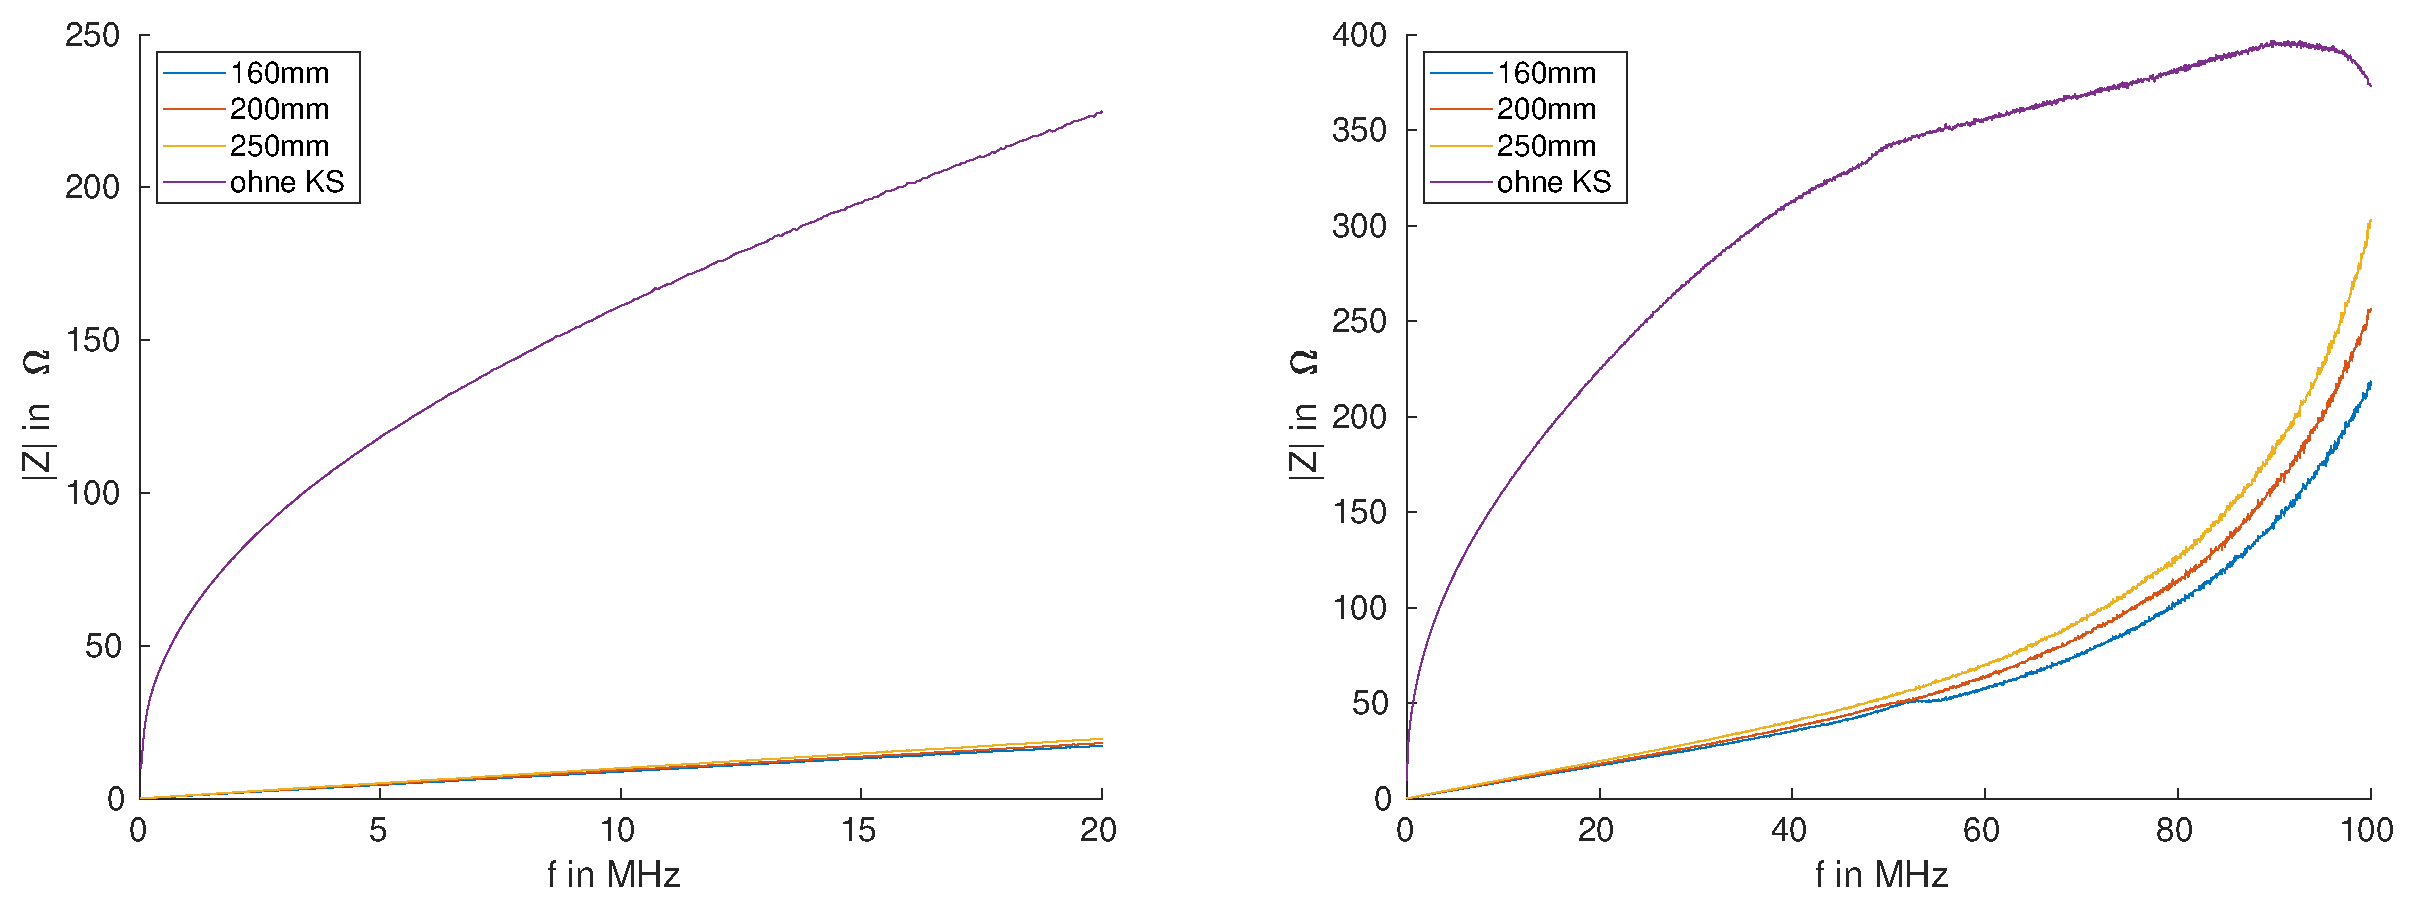
\includegraphics[width=\textwidth]{Z_RK_length_2KS}}
	\caption{Gegen\"uberstellung der Ringkernimpedanz f\"ur verschiedene L\"angen der Kurzschl\"usse.}
	\label{fig:ringcoreheight}
\end{figure}

Es f\"allt auf, dass der Effekt von l\"angeren Kurzschl\"ussen besonders im unteren Frequenzbereich noch deutlich geringer ausf\"allt, als es bei der Breitenvariation der Fall ist. Um das genauer Quantifizieren zu k\"onnen werden auch hier f\"ur Frequenzen von 5, 10 und $\SI{20}{\mega\hertz}$ die Ringkernimpedanz \"uber der L\"ange der Kurzschl\"usse aufgetragen. Das Ergebnis ist in Abbildung~\ref{fig:ringcoreheight20} zu sehen.




\newpage



\begin{figure}[htb]
	\centering
	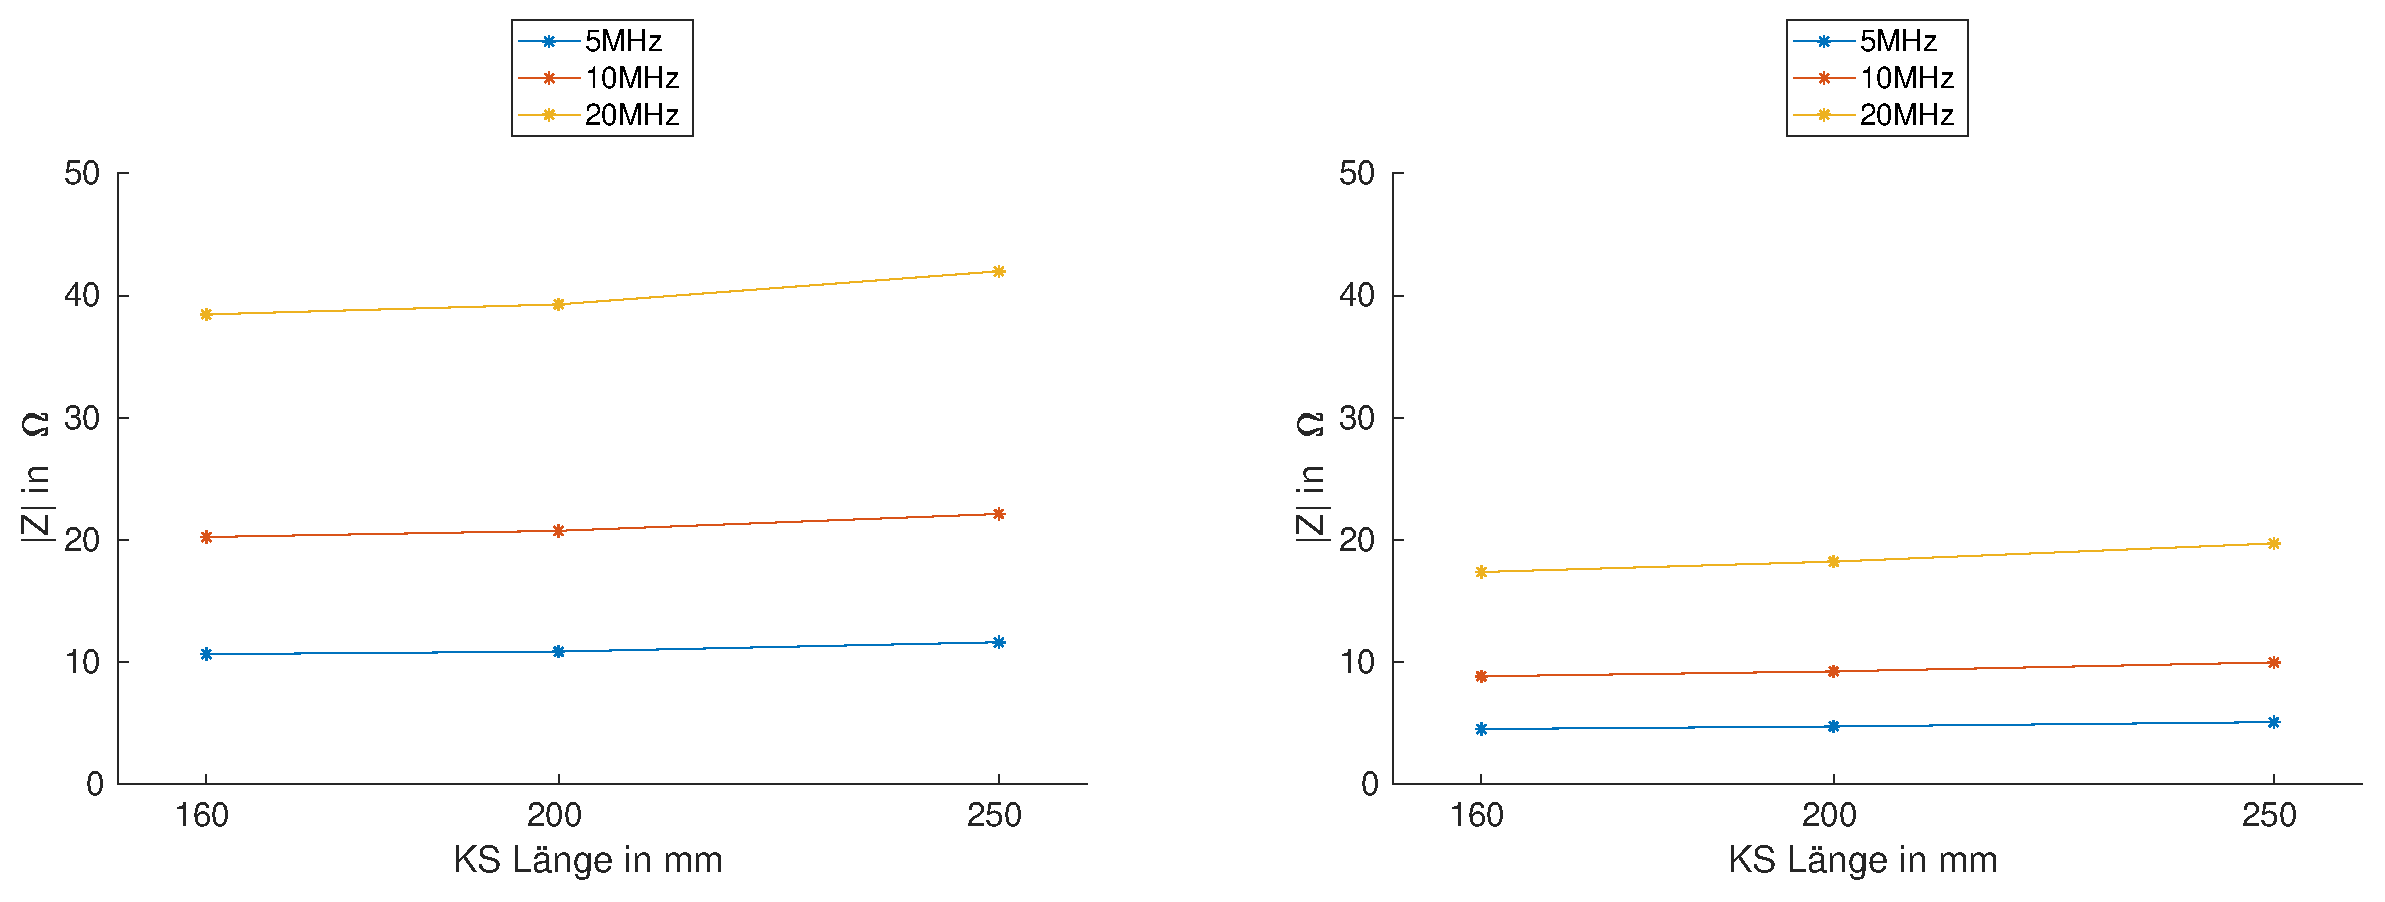
\includegraphics[width=\textwidth]{RK_Impedanz_length_frequenz}
	\caption{Gegen\"uberstellung der Ringkernimpedanz bei 5, 10 und $\SI{20}{\mega\hertz}$. Links: 1KS, rechts: 2KS.}
	\label{fig:ringcoreheight20}
\end{figure}

Der Extremfall ist hier die Variation bei $\SI{20}{\mega\hertz}$ und zwei Kurzschl\"ussen zwischen $\SI{160}{\milli\meter}$ und $\SI{250}{\milli\meter}$ L\"ange. Setzt man die Werte in Gleichung~\ref{eq:maxdiffpercent} ein, so erh\"alt man eine Abweichung von rund $\SI{1,3}{\%}$. 

\subsection{Dicke der Kurzschl\"usse}
Die Variation der Dicke ist in der Fertigung etwas aufwendiger. Zun\"achst m\"ussen die B\"ugel aus einem anderen Blech geschnitten werden. insbesondere das Biegen der B\"ugel gestaltet sich hierbei aber schwierig, da die zunehmende Dicke der Bleche das Biegen erschweren und h\"ohere Dicken anderes Werkzeug erforderten. Daher ist dieser Variationsparameter nur f\"ur zwei Dicken, n\"amlich $\SI{1}{\milli\meter}$ und $\SI{2}{\milli\meter}$ vorgesehen worden.
\par
Die Auftragung der Ringkernimpedanz \"uber der Frequenz liefert das in Abbildung~\ref{fig:ringcorethick} gezeigte Ergebnis.



\newpage




\begin{figure}[htb]
	\centering
	\subfloat[1 Kurzschluss]{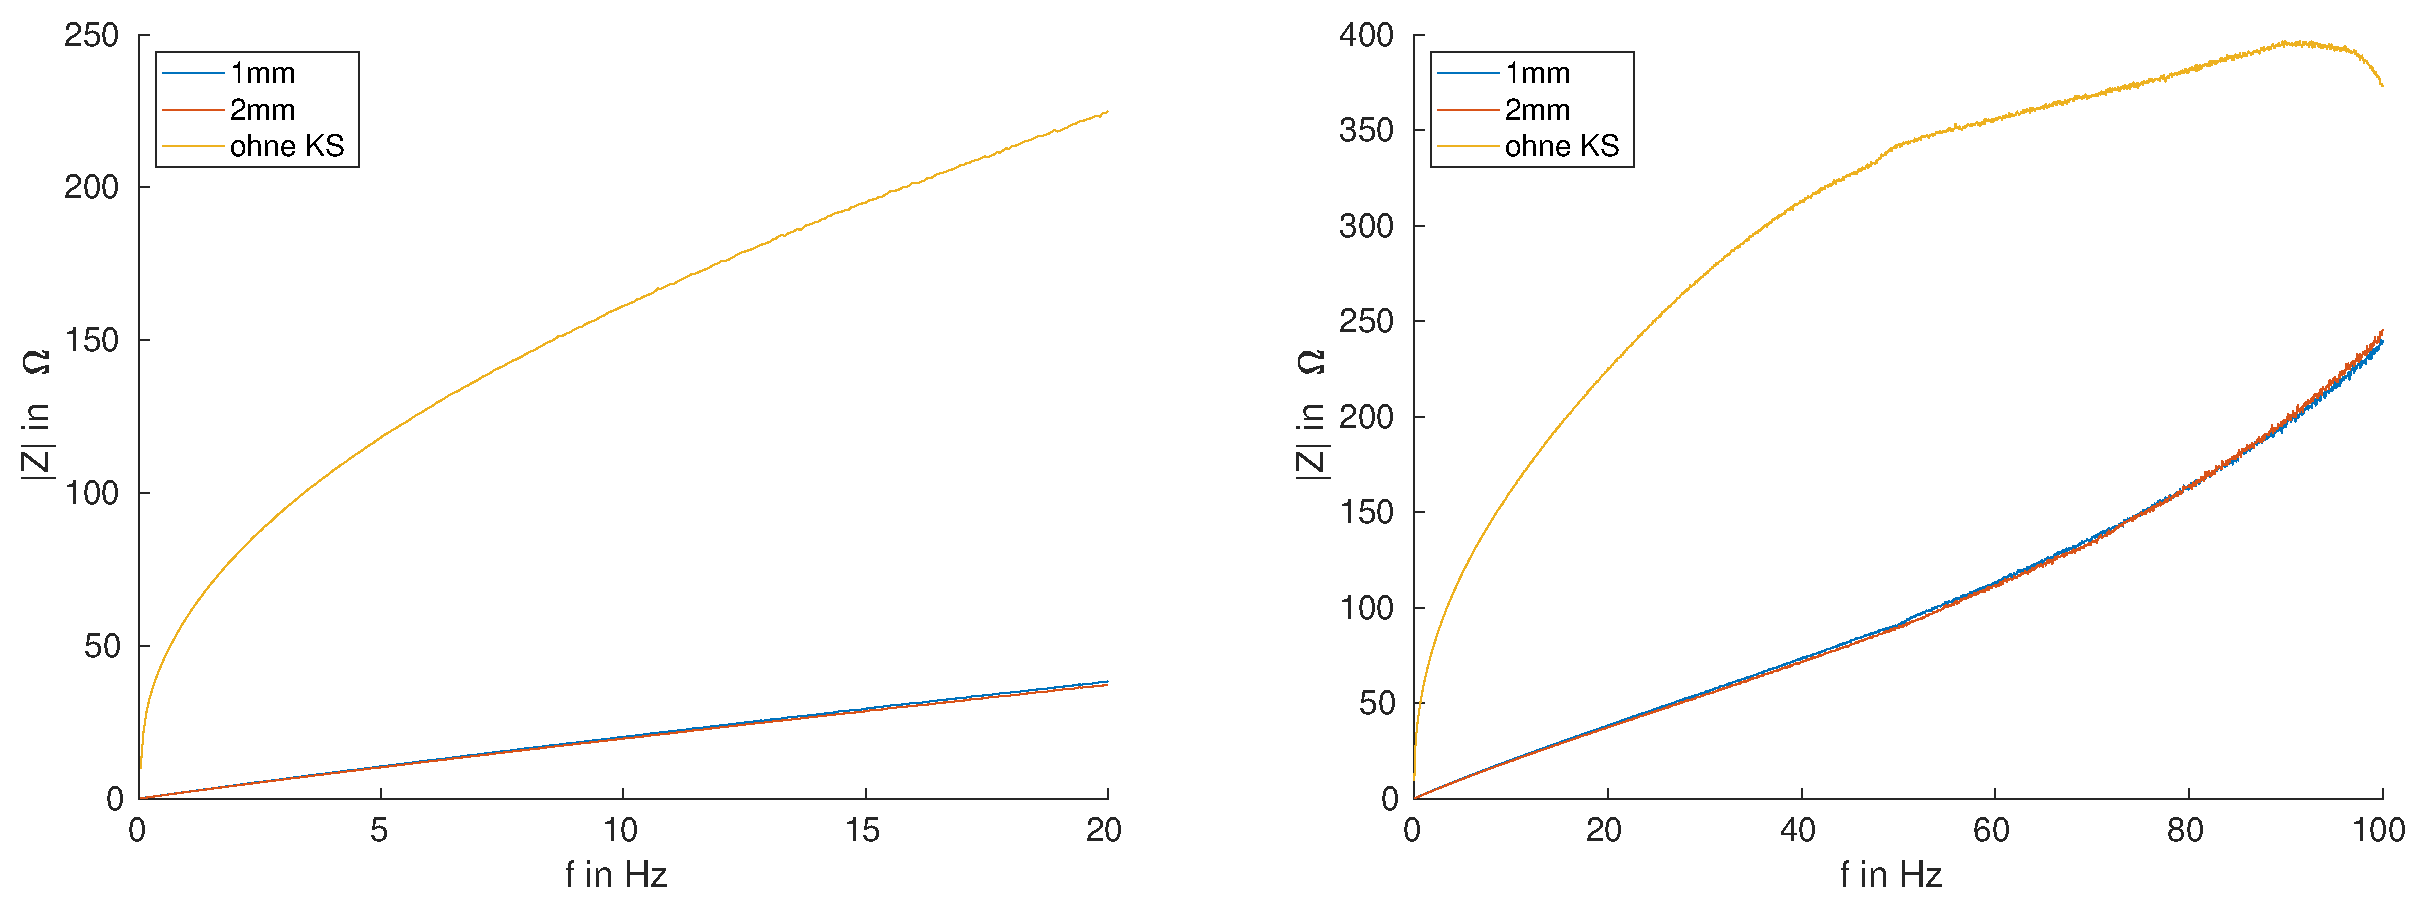
\includegraphics[width=\textwidth]{Z_RK_thick_1KS}}
	\\
	\subfloat[2 Kurzschl\"usse]{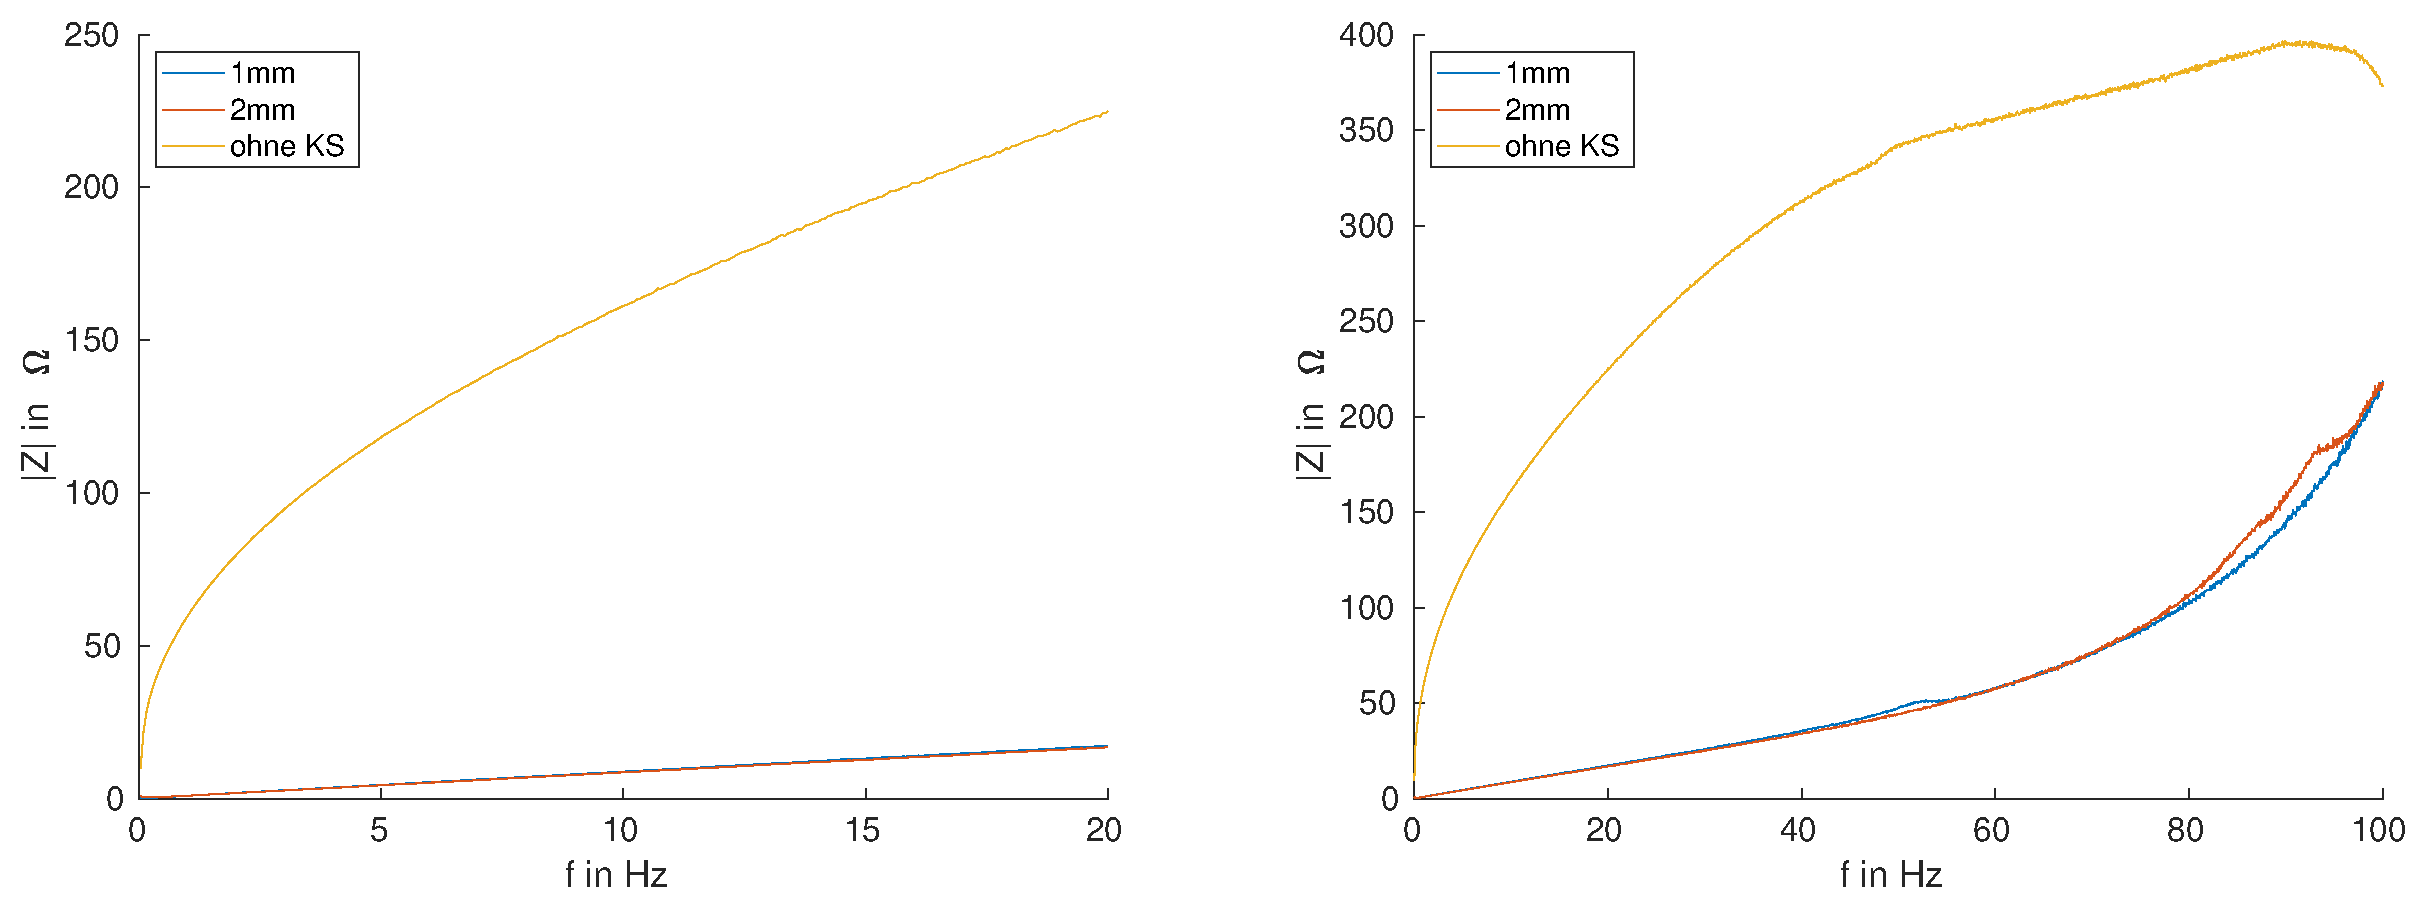
\includegraphics[width=\textwidth]{Z_RK_thick_2KS}} 
	\caption{Gegen\"uberstellung der Ringkernimpedanz f\"ur verschiedene Dicken der Kurzschl\"usse.}
	\label{fig:ringcorethick}
\end{figure}

Da nur zwei Stufen f\"ur die Dicke gemessen wurden, wird in diesem Fall auf eine Grafik f\"ur die einzelnen Frequenzpunkte verzichtet. Die Berechnung der Abweichung f\"ur den Vergleich von zwei Kurzschl\"ussen bei $\SI{20}{\mega\hertz}$ mit verschiedenen Dicken liefert nach Gleichung~\ref{eq:maxdiffpercent} einen prozentualen Wert von $\SI{0,286}{\%}$. 
Die Dicke des Blechs hat damit nahezu keinen Einfluss auf die Ringkernimpedanz.



\newpage